\section{Cuantificadores de la teoría de la información}
\label{sec:ITQs}

Dada una fuente de símbolos cuya salida es un vector de símbolos $X$, existen diferentes procedimientos para obtener una PDF \cite{Rosso2009, DeMicco2008, Mischaikow1999, Powell1979, Rosso2001, Pompe2002}.
La determinación de la mejor PDF $P$ es un problema fundamental porque $P$ y el espacio de muestra $X$ están inextricablemente vinculados.
Su aplicabilidad depende de las características particulares de los datos, tales como estacionariedad, duración de la serie temporal, variación de los parámetros, nivel de contaminación de ruido, etc.

Los cuantificadores seleccionados se basan en el recuento de símbolos y en la estadística de patrones de orden.
Las métricas a utilizar pueden clasificarse de forma amplia en dos categorías: las que cuantifican el \textit{contenido de información} de los datos en comparación con los relacionados con su \textit{complejidad}.
Obsérvese que aquí nos estamos refiriendo al espacio de funciones de densidad de probabilidad, no al espacio físico.
Para clarificar y simplificar, introducimos solamente los cuantificadores de la Teoría de la Información que se definen en PDFs discretas, ya que solo estamos tratando con datos discretos (series temporales).
Sin embargo, todos los cuantificadores también tienen definiciones para el caso continuo \cite{Shannon1948}.

\subsection{Entropía de Shannon y Complejidad Estadística}

La entropía es una cantidad básica que puede considerarse como una medida de la incertidumbre asociada (información) al proceso físico descrito por $P$.
Al tratar con el contenido de la información, la entropía de Shannon se considera a menudo como la fundamental y más natural \cite{Shannon1948}.
Considerada como una medida de la incertidumbre, es el ejemplo más paradigmático de estos cuantificadores de información.

Sea $P=\{p_i; i=1,\ldots, N\}$ con $\sum_{i=1}^N p_i = 1$, una distribución de probabilidad discreta, con $N$ el número de estados posibles del sistema bajo estudi.
La medida de la información logarítmica de shannon se denota como
\begin{equation}
\label{Shannon-disc}
S[P] ~=~ -\sum_{i=1}^{N} p_i \ln \left[ p_i \right] \ .
\end{equation}

Si $S[P] = S_{\min} = 0$, estaremos en posición de predecir con total certeza cuáles de los posibles resultados $i$, cuyas probabilidades están dadas por $p_i$, tendrán lugar realmente.
Nuestro conocimiento del proceso subyacente descrito por la distribución de probabilidad es máximo en este caso.
Por el contrario, nuestro conocimiento es mínimo para una distribución uniforme $P_e = \{p_i = 1/N; i = 1, \ldots, N \}$ dado que cada resultado exhibe la misma probabilidad de ocurrencia, y la incertidumbre es máxima, es decir, $S[P_e] = S_{\ max} = \ln N$.
Estas dos situaciones son casos extremos, por lo tanto nos centramos en la entropía de Shannon "normalizada", $0 \leq H \leq 1$, dada como
\begin{equation}
\label{shannon-disc-normalizada}
H[P] = S[P] / S_{\max} \ .
\end{equation}

Contrariamente al contenido de la información, no existe una definición universalmente aceptada de complejidad.
Aquí, nos centramos en describir la \textit{complejidad de las series temporales} y no nos referimos a la complejidad de los \textit{sistemas} subyacentes.
Un sistema complejo no genera necesariamente una salida compleja.
De hecho, los modelos "simples" pueden generar datos complejos, mientras que los sistemas "complicados" pueden producir datos de salida de baja complejidad \cite{Kantz1998}.

Una noción intuitiva de una complejidad cuantitativa atribuye valores bajos tanto a datos perfectamente ordenados (es decir, con entropía de Shannon que se va desapareciendo) como a datos aleatorios no correlacionados (con entropía Shannon máxima).
Por ejemplo, la complejidad estadística de una simple oscilación o tendencia (ordenada), pero también de ruido blanco no correlacionado (no ordenado) sería clasificada como baja.
Entre los dos casos de mínima y máxima entropía, los datos son más difíciles de caracterizar y por lo tanto la complejidad debe ser mayor.
Buscamos alguna función $C[P]$ que cuantifique las estructuras presentes en los datos que se alejan de estos dos casos.
Estas estructuras se relacionan con la organización, la estructura correlacional, la memoria, la regularidad, la simetría, los patrones y otras propiedades \cite{Feldman2008}.

Asumimos que el grado de estructuras correlacionales sería capturado adecuadamente por algún funcional $C[P]$ de la misma manera que la entropía de Shannon $S[P]$ \cite{Shannon1948} ``capta " la aleatoriedad.
Claramente, las estructuras ordinales presentes en un proceso no son cuantificadas por medidas de aleatoriedad y, por consiguiente, son necesarias medidas de complejidad estadística o estructural para una mejor comprensión (caracterización) de la dinámica del sistema representada por sus series temporales \cite{Feldman1998}.

Una medida adecuada de complejidad puede definirse como el producto de una medida de información y una medida de desequilibrio, es decir, algún tipo de distancia de la distribución equiprobable de los estados accesibles de un sistema.
En este sentido, en \cite{Lamberti2004} los autores introdujeron una eficaz {\it Medida de Complejidad Estadística \/} (SCM) $C$, que es capaz de detectar detalles esenciales de los procesos dinámicos subyacentes al conjunto de datos.
Basado en el trabajo de López-Ruiz \cite{Lopez1995}, esta medida de complejidad estadística \cite{Martin2003,Lamberti2004} se define a través de la forma del producto
\begin{equation}
C[P] = Q_{J}[P,P_e] \cdot H[P]
\label{complexity}
\end{equation}
de la entropía de Shannon normalizada $H$, ver eq. \eqref{shannon-disc-normalizada}, y el desequilibrio $Q_{J}$ definido en términosde la divergencia de Jensen-Shannon $J[P, P_e]$.
Esto es,
\begin{equation}
\label{disequilibrium}	
Q_{J} [ P, P_e] = Q_{0} J[ P, P_e] = Q_{0} \{ S[(P + P_e)/2 ] - S[ P ]/2 - S[P_e]/2\},
\end{equation}
en la divergencia de Jensen-Shannon mencionada arriba, $Q_0$ es una constante de normalización tal que $0 \leq Q_{J} \leq 1$:
\begin{equation}
Q_0 ~=~ -2 \left\{ {\frac{N+1}{N}} \ln (N+1) - \ln (2N) + \ln N \right\}^{-1} \ ,
\label{q0-jensen-1}
\end{equation}
y es igual a la inversa del máximo valor posible de $J [P,P_e]$.
Este valor es obtenido cuando una de las componentes de $P$, digamos $p_m$, es igual a uno y todos los $p_j$ restantes son cero.

La divergencia de Jensen-Shannon, que cuantifica la diferencia entre las distribuciones de probabilidad, es especialmente útil para comparar la composición simbólica entre diferentes secuencias \cite{Grosse2002}.
Obsérvese que la SCM introducida anteriormente depende de dos distribuciones de probabilidad diferentes: una asociada con el sistema analizado, $P$, y la otra con la distribución uniforme, $P_e$.
Además, se demostró que para un valor dado de $H$, el rango de valores posibles de $C$ varía entre un mínimo $C_ {min}$ y un máximo $C_ {max}$, restringiendo los posibles valores del SCM \cite{Martin2006}.

Por lo tanto, está claro que información adicional importante relacionada con la estructura correlacional entre los componentes del sistema físico se proporciona evaluando la medida de la complejidad estadística.

\subsection{Determinación de la distribución de probabilidad}

La evaluación de los cuantificadores derivados de la Teoría de la Información supone algún conocimiento previo sobre el sistema; específicamente para aquellos introducidos previamente (entropía de Shannon y complejidad estadística), una distribución de probabilidad asociada a la serie temporal en análisis debe proporcionarse antes.
La determinación del PDF más adecuado es un problema fundamental porque la PDF $P$ y el espacio de muestra $\Omega$ están intrincadamente vinculados.

Las metodologías usuales asignan a cada valor de la serie $X(t)$ (o conjunto de valores consecutivos no superpuestos) un símbolo de un alfabeto finito $A = \{a_1, \dots, a_M \}$, creando así una {\it secuencia simbólica \/} que puede considerarse como una descripción de la serie cronológica en cuestión.
Como consecuencia, las relaciones de orden y las escalas temporales de la dinámica se pierden por completo.

Es importante resltar que $P$ en si, no es un objeto con una definición única y existen varias aproximaciones para ``asociar'' una dada $P$ con una dada serie de tiempo.
Solo para mencionar algunos criterios de extracción utilizados frecuentemente en la literatura: {\it a)\/} histogramas de series temporales \cite{Martin2004}, {\it b)\/} dinámica simbólica binaria \cite{Mischaikow1999}, {\it c)\/} análisis de Fourier \cite{Powell1979}, {\it d)\/} trensformadas wavelet \cite{Blanco1998,Rosso2001}, {\it e)\/} PDF de particiones \cite{Ebeling2001}, {\it f)\/} PDF de permutaciones \cite{Pompe2002,Keller2005}, {\it g)\/} PDF discreta \cite{Amigo2007}, etc.
Hay una amplia libertad para elegir entre ellas y la aplicación específica debe ser analizada para hacer una buena elección.

Se puede incorporar debidamente la información causal si se incluye información sobre la dinámica pasada del sistema en la secuencia simbólica, es decir, los símbolos del alfabeto $A$ se asignan a una porción del espacio de fase o trayectoria.
Bandt y Pompe (BP) \cite{Bandt2002} introdujeron una metodología simbólica simple y robusta que toma en cuenta el ordenamiento temporal de las series temporales comparando valores vecinos en una serie temporal.
La propiedad de causalidad de la PDF permite que los cuantificadores (basados en esta PDF) discriminan entre sistemas determinísticos y estocásticos \cite{Rosso2007B}.
Los datos simbólicos son:
{\it (i) \/} ~ creados por la clasificación de los valores de la serie; y
{\it (ii) \/} ~ definidos por el reordenaminto de los datos embebidos en orden ascendente, lo que equivale a una reconstrucción de espacio de fase con dimensión de emmbedding (longitud de patrón) $D$ y retardo de tiempo $\tau$.
De esta forma, es posible cuantificar la diversidad de los símbolos de ordenación (patrones) derivados de una serie temporal escalar.
Obsérvese que la secuencia de símbolos apropiada surge naturalmente de la serie temporal, y no se necesitan suposiciones basadas en modelos.
El procedimiento es el siguiente:
\begin{itemize}
	\item Dada una serie $\{x_t; t=0, \Delta t, \cdots,N\Delta t \}$, se genera una secuencia de vectores de longitud $D$.
	\begin{equation}
	(s)\longmapsto\left(x_{t-(d-1)\Delta t},x_{t-(d-2)\Delta t},\dots,x_{t-\Delta t},x_{t}\right) 
	\label{eq:vectores}
	\end{equation}
	Cada vector resulta ser la "historia" del valor $x_t$. Evidentemente, cuanto más larga sea la longitud de los vectores $D$, mayor será la información sobre la historia de los vectores, pero se requiere un valor más alto de $N$ para tener una estadística adecuada.
	\item Las permutaciones $\pi=(r_0, r_1, \cdots, r_{D-1})$ de $(0, 1, \cdots, D-1)$ es llamado ``patrón de orden'' de tiempo $t$, definido por:
	\begin{equation}
	\label{eq:permuta}
	x_{t-r_{D-1}\Delta t}\le x_{t-r_{D-2}\Delta t}\le\dots\le x_{t-r_{1}\Delta t}\le x_{t-r_0\Delta t}
	\end{equation}
	Para obtener se un resultado único se considera $r_i<r_{i-1}$ si $x_{t-r_{i}\Delta t}=x_{t-r_{i-1}\Delta t}$.
	De esta forma, todas las $D!$ permutaciones posibles $\pi$ de orden $D$, y la PDF $P=\{p(\pi)\}$ es definida como:
	\begin{equation}
	\label{eq:frequ}
	p(\pi)=\frac{\sharp \{s|s\leq N-D+1; (s) \quad \texttt{has type}~\pi\}}{N-D+1}
	\end{equation}
	En estas últimas expresiones, el símbolo $\sharp$ denota cardinalidad.
\end{itemize}

Por lo tanto, una distribución de probabilidad de patrones de órden $P = \{ p(\pi_i), i = 1, \dots, D! \}$ se obtiene de la serie temporal.
De esta manera, el vector definido por la ecuación \eqref{eq:frequ} se convierte en un símbolo único $\pi$.
Se establece $r_i < r_{i-1}$ si $x_{s-r_{i}} = x_{s-r_{i-1}}$ para la obtener una única solución.
La única condición para la aplicabilidad del método BP es una suposición estacionaria muy débil: para $k \leq D$, la probabilidad para $x_t<x_{t + k}$ no debe depender de $t$.
Con respecto a la selección de los parámetros, Bandt y Pompe sugirieron trabajar con $3 \leq D \leq 6$ para longitudes de series de tiempo típicas, y específicamente se consideró un retraso de tiempo $\tau = 1$ en su publicación principal.

Para destacar la diferencia entre una $P$ \textit{causal} y una \textit{no causal}, consideremos una serie de valores $X=\{x_i,~i=1,2,...\}$ generada por la función $randn$ de Matlab's $^\copyright$; consideremos también la serie $Y=\{y_i,~i=1,2,...\}$ como la resultante de ordenar la serie $X$ en forma ascendente. Esto se puede ver en el ejemplo en la figura \ref{fig:causal_nocausal}, en la figura \ref{subfig:causal_nocausal_x} se muestran 1000 valores sorteados con una distribución uniforme entre 0 y 1, también mostramos en la figura \ref{subfig:causal_nocausal_y} la versión ordenada de la serie de la figura \ref{subfig:causal_nocausal_x}, son los mismos valores pero ordenados en forma ascendente. Una $P$ no causal es el histograma normalizado que mostramos en las figuras \ref{subfig:causal_nocausal_HistValx} y \ref{subfig:causal_nocausal_HistValy}, en donde puede verse que $P(X)$ es idéntica a $P(Y)$, por lo que todos los cuantificadores que se calculen a partir de ellas serán idénticos para las dos series. Una $P$ causal puede ser obtenida mediante el procedimiento de Bandt \& Pompe descripto arriba, en este caso $P(X)$ de la figura \ref{subfig:causal_nocausal_HistBPx} es bastante uniforme y $P(Y)$ de la figura \ref{subfig:causal_nocausal_HistBPy} tiene una forma tipo delta. En este caso, $P$ registra que $Y$ es monótonamente creciente y presenta un solo patrón de orden.

\begin{figure}[htpb]
	\centering
	\begin{subfigure}[t]{0.49\textwidth}
		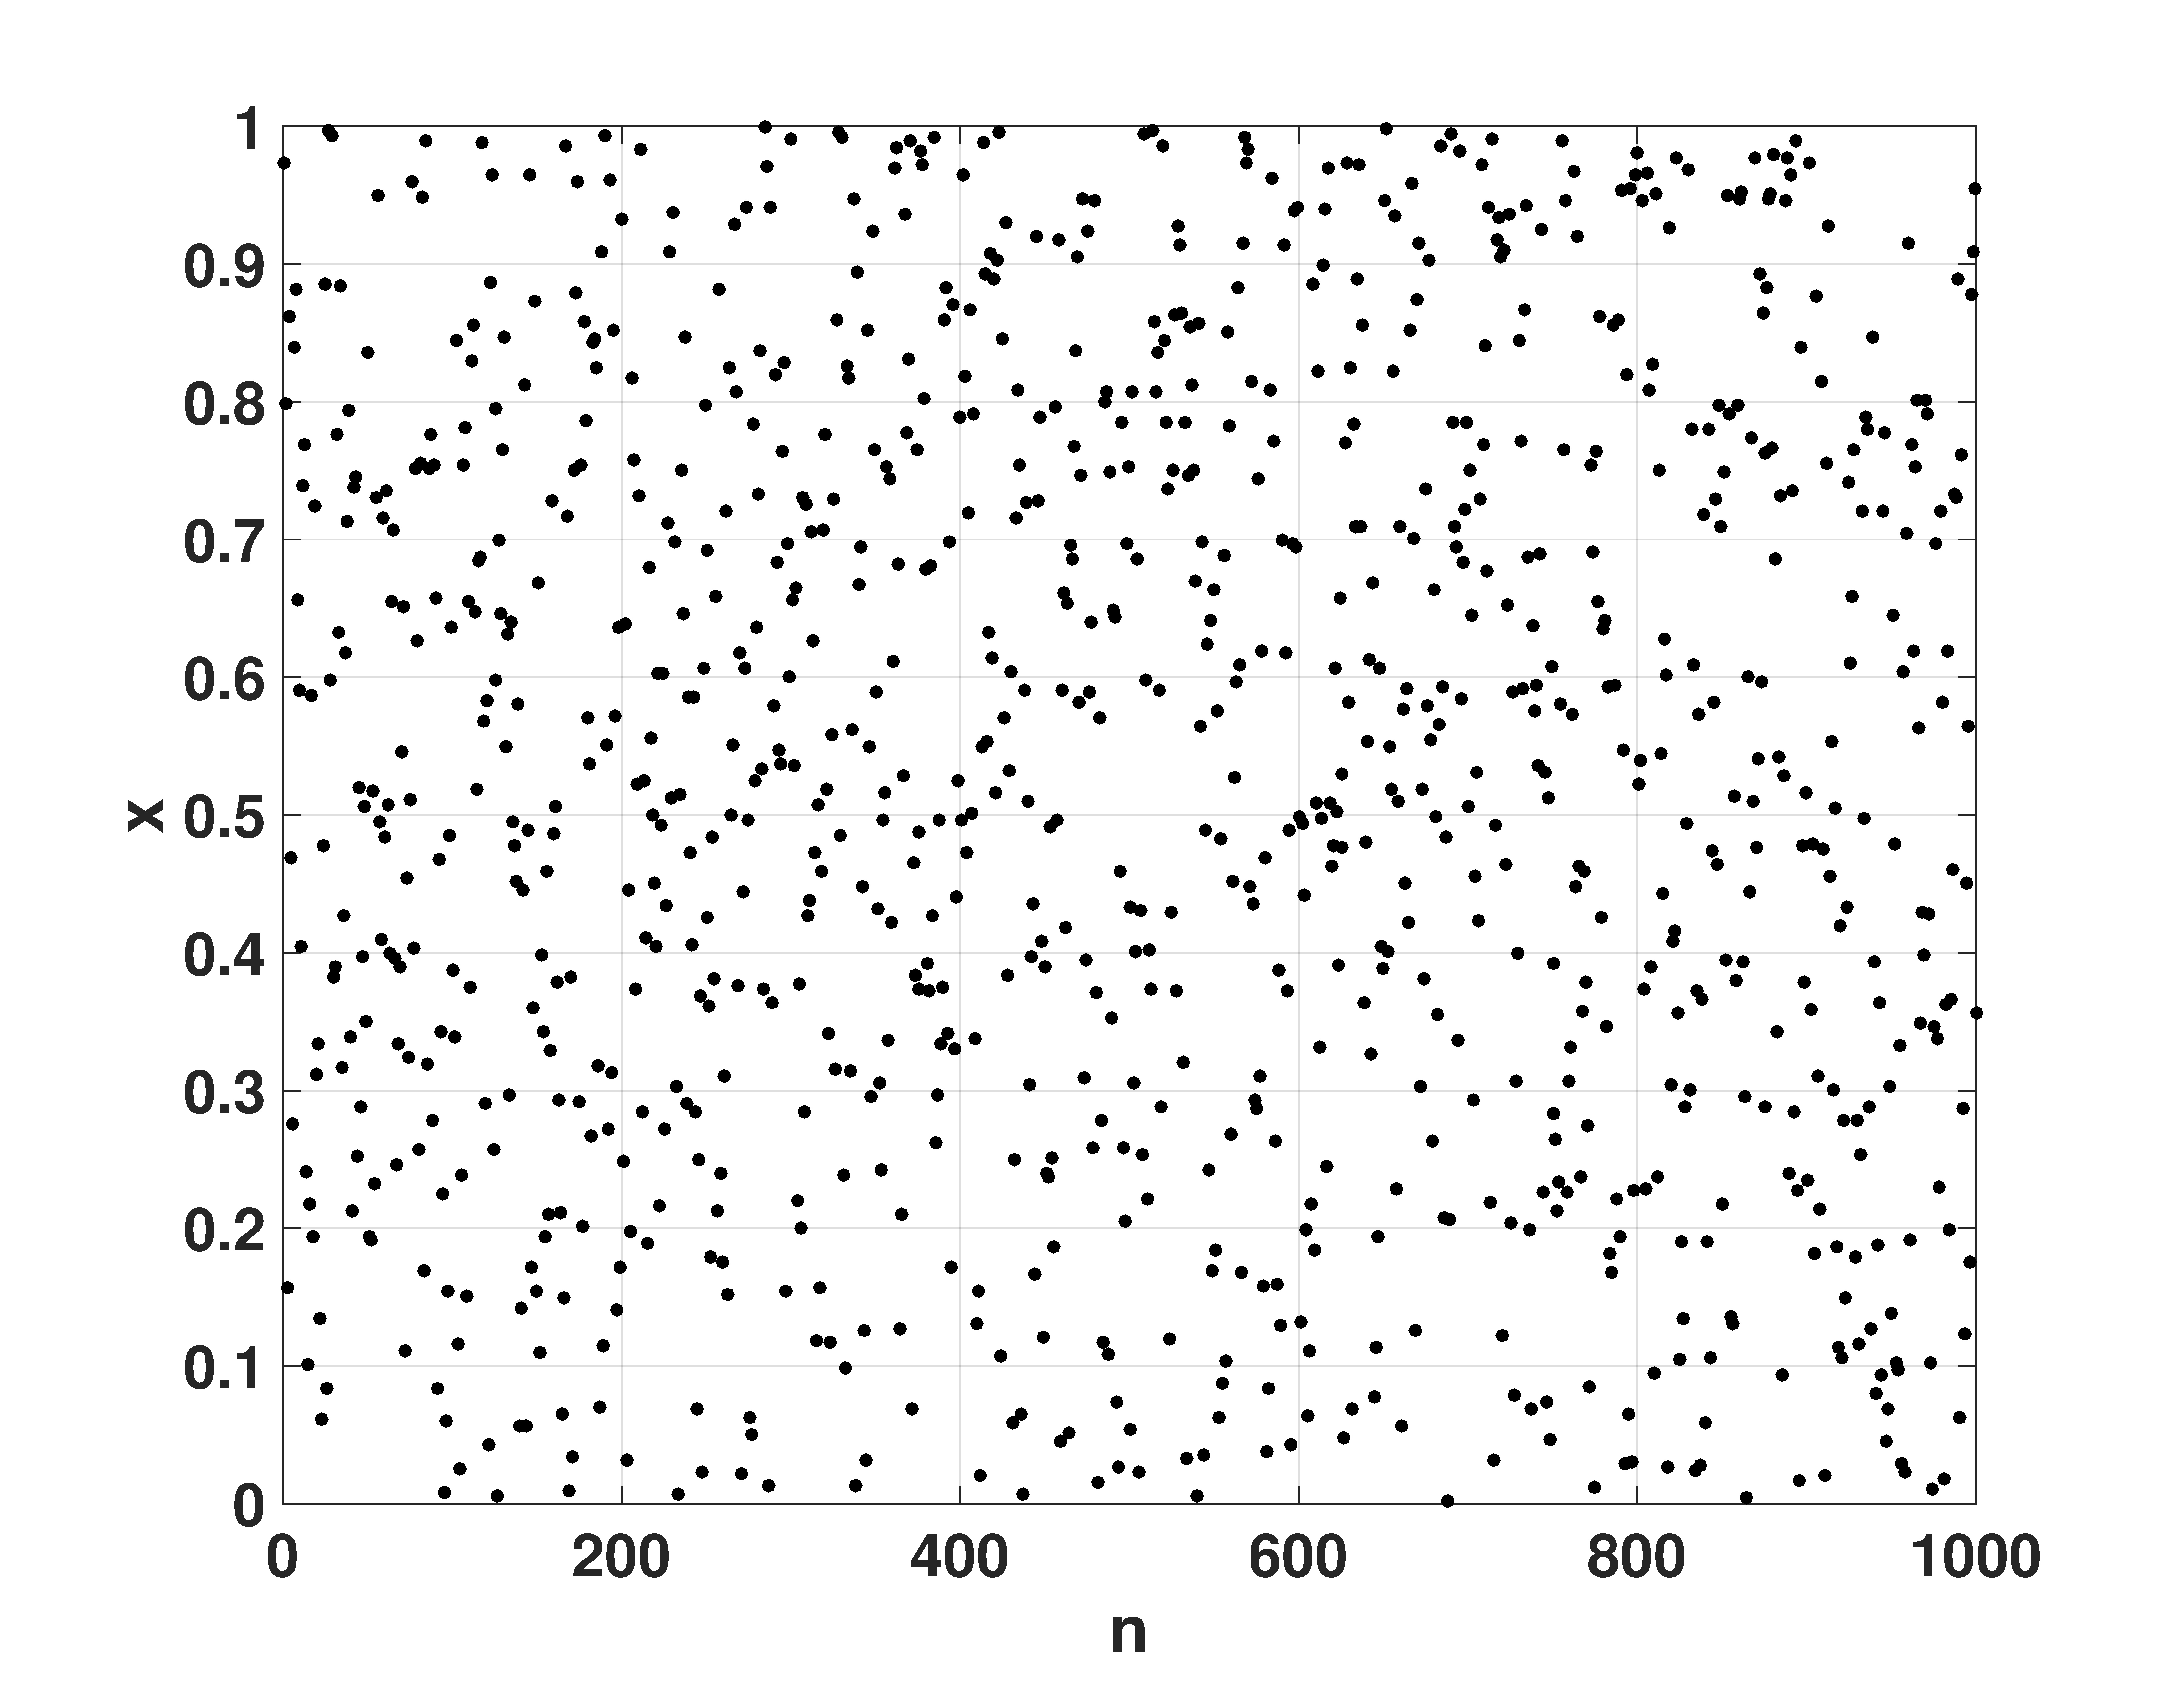
\includegraphics[width=\textwidth]{x}
		\caption{$1000$ puntos con distribución uniforme}
		\label{subfig:causal_nocausal_x}
	\end{subfigure}
	\begin{subfigure}[t]{0.49\textwidth}
		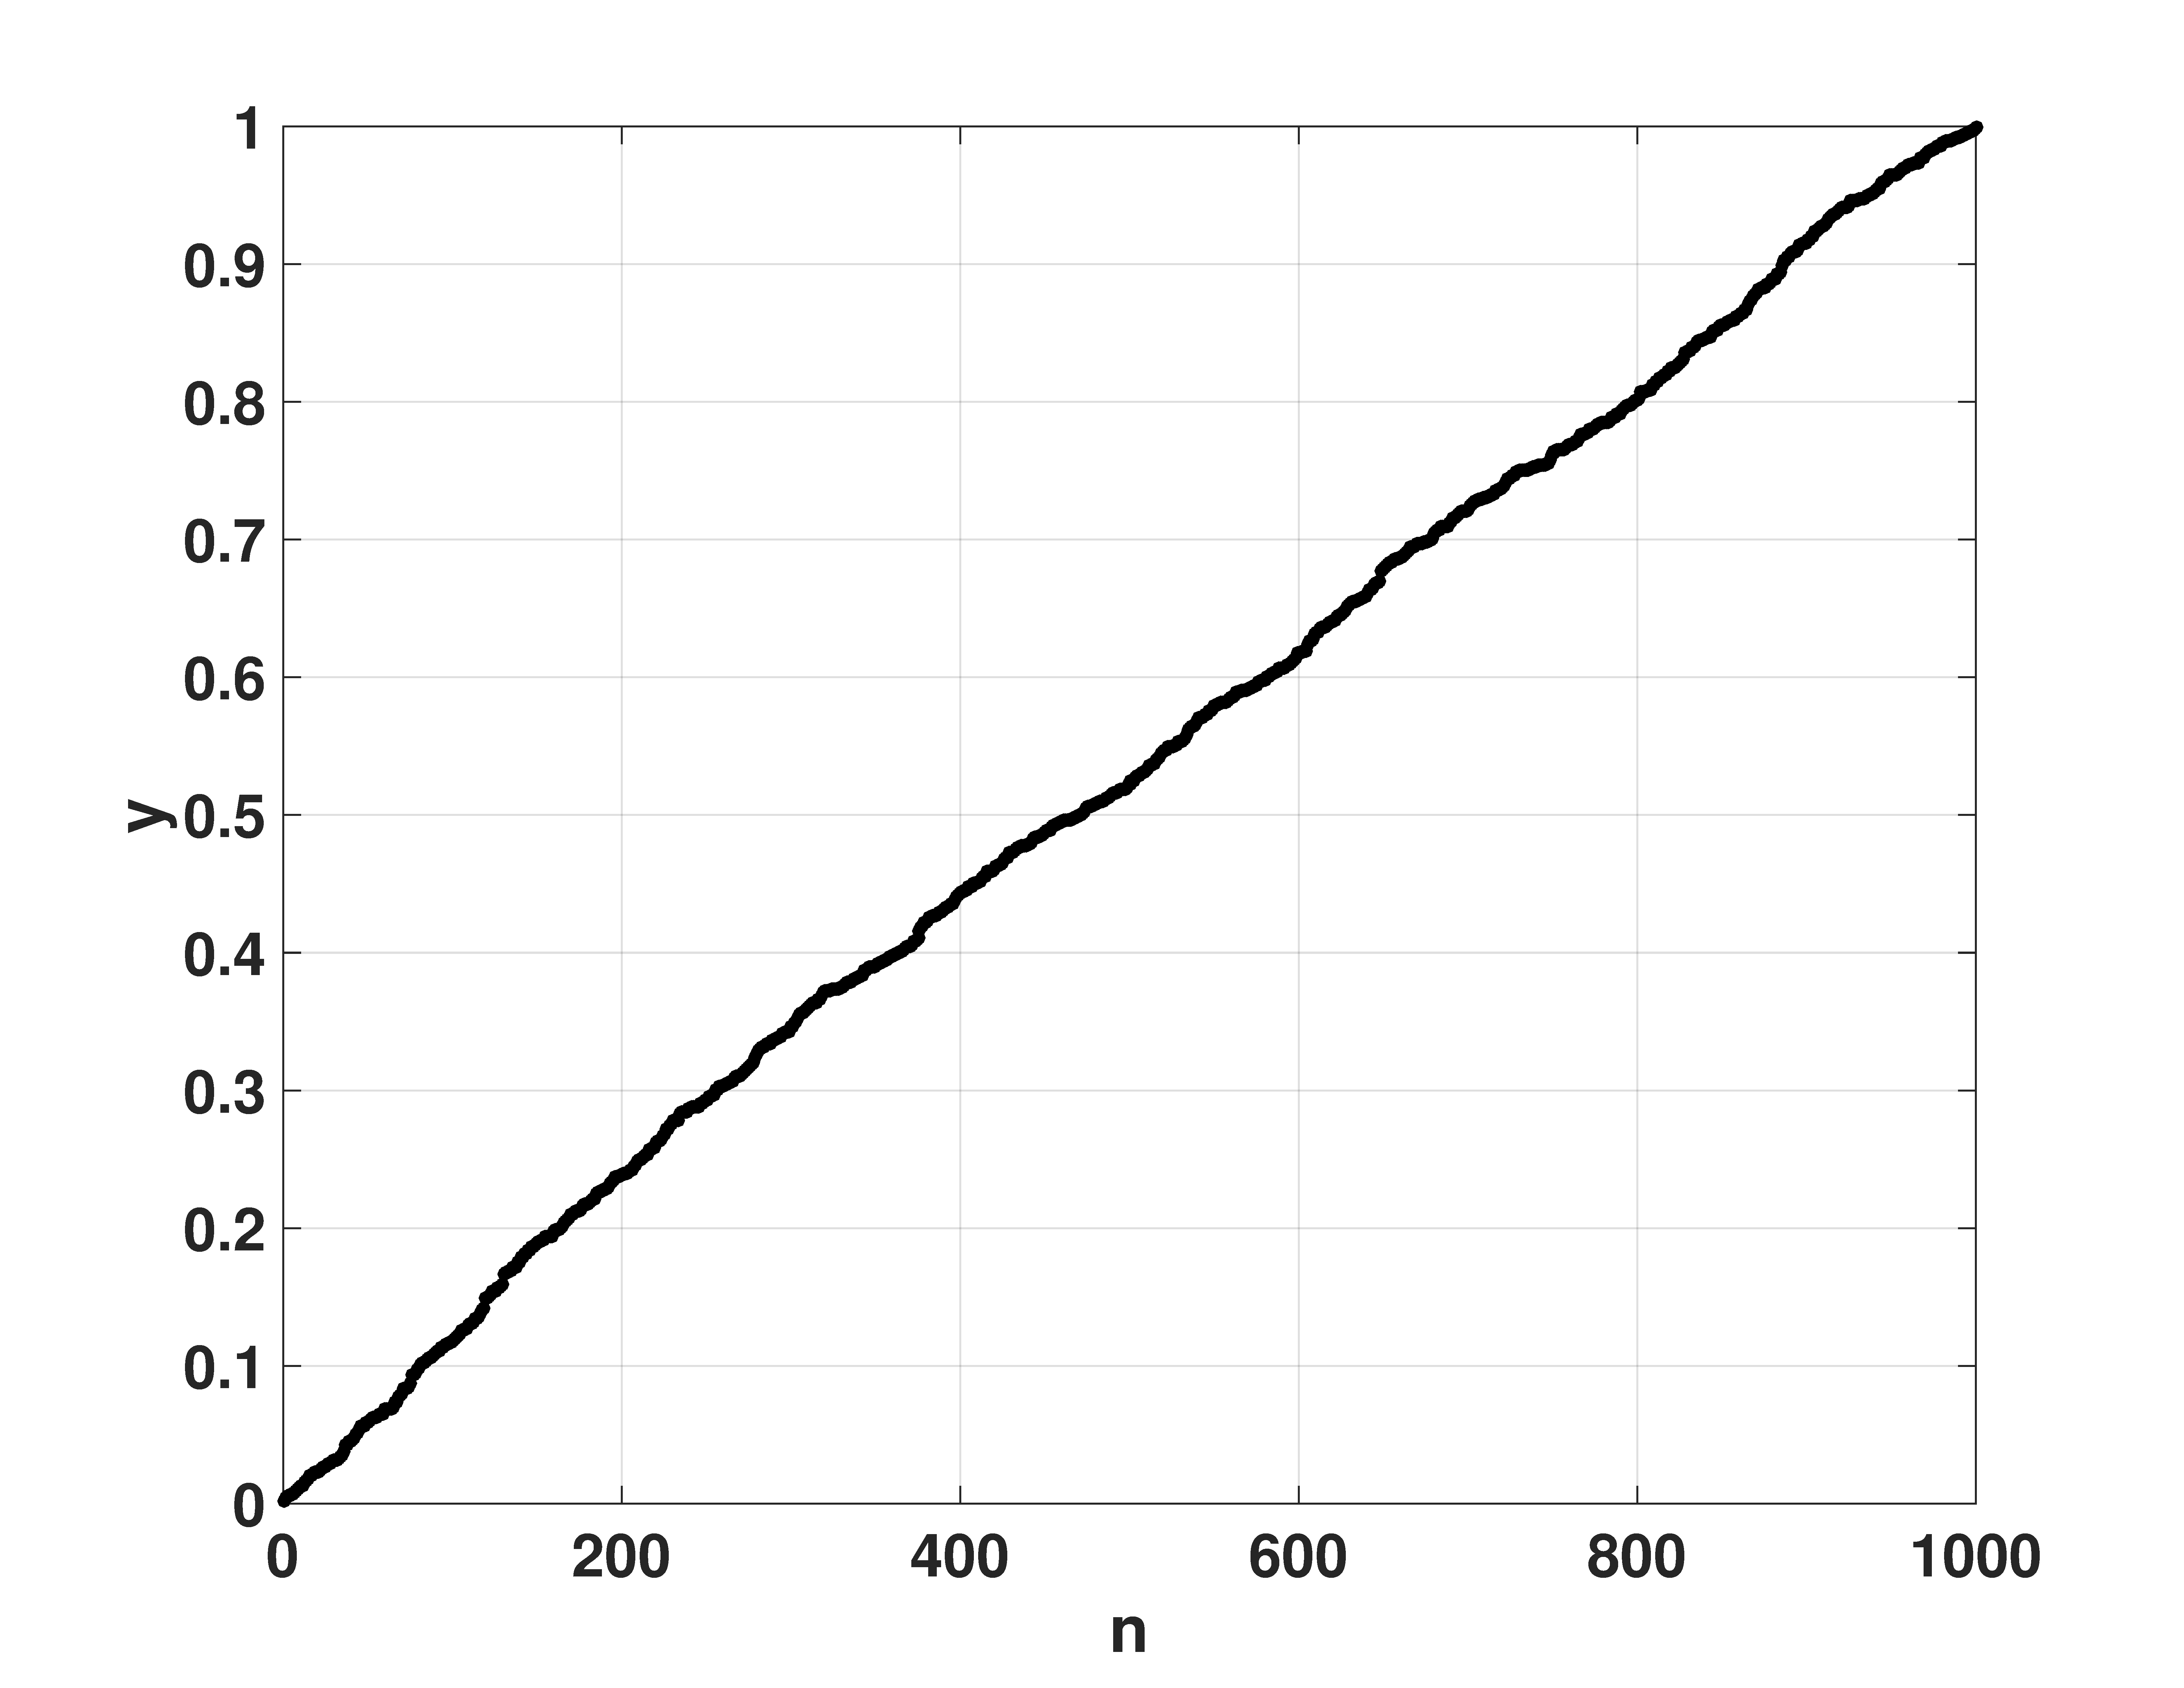
\includegraphics[width=\textwidth]{y}
		\caption{Puntos ordenados}
		\label{subfig:causal_nocausal_y}
	\end{subfigure}
	\begin{subfigure}[t]{0.49\textwidth}
		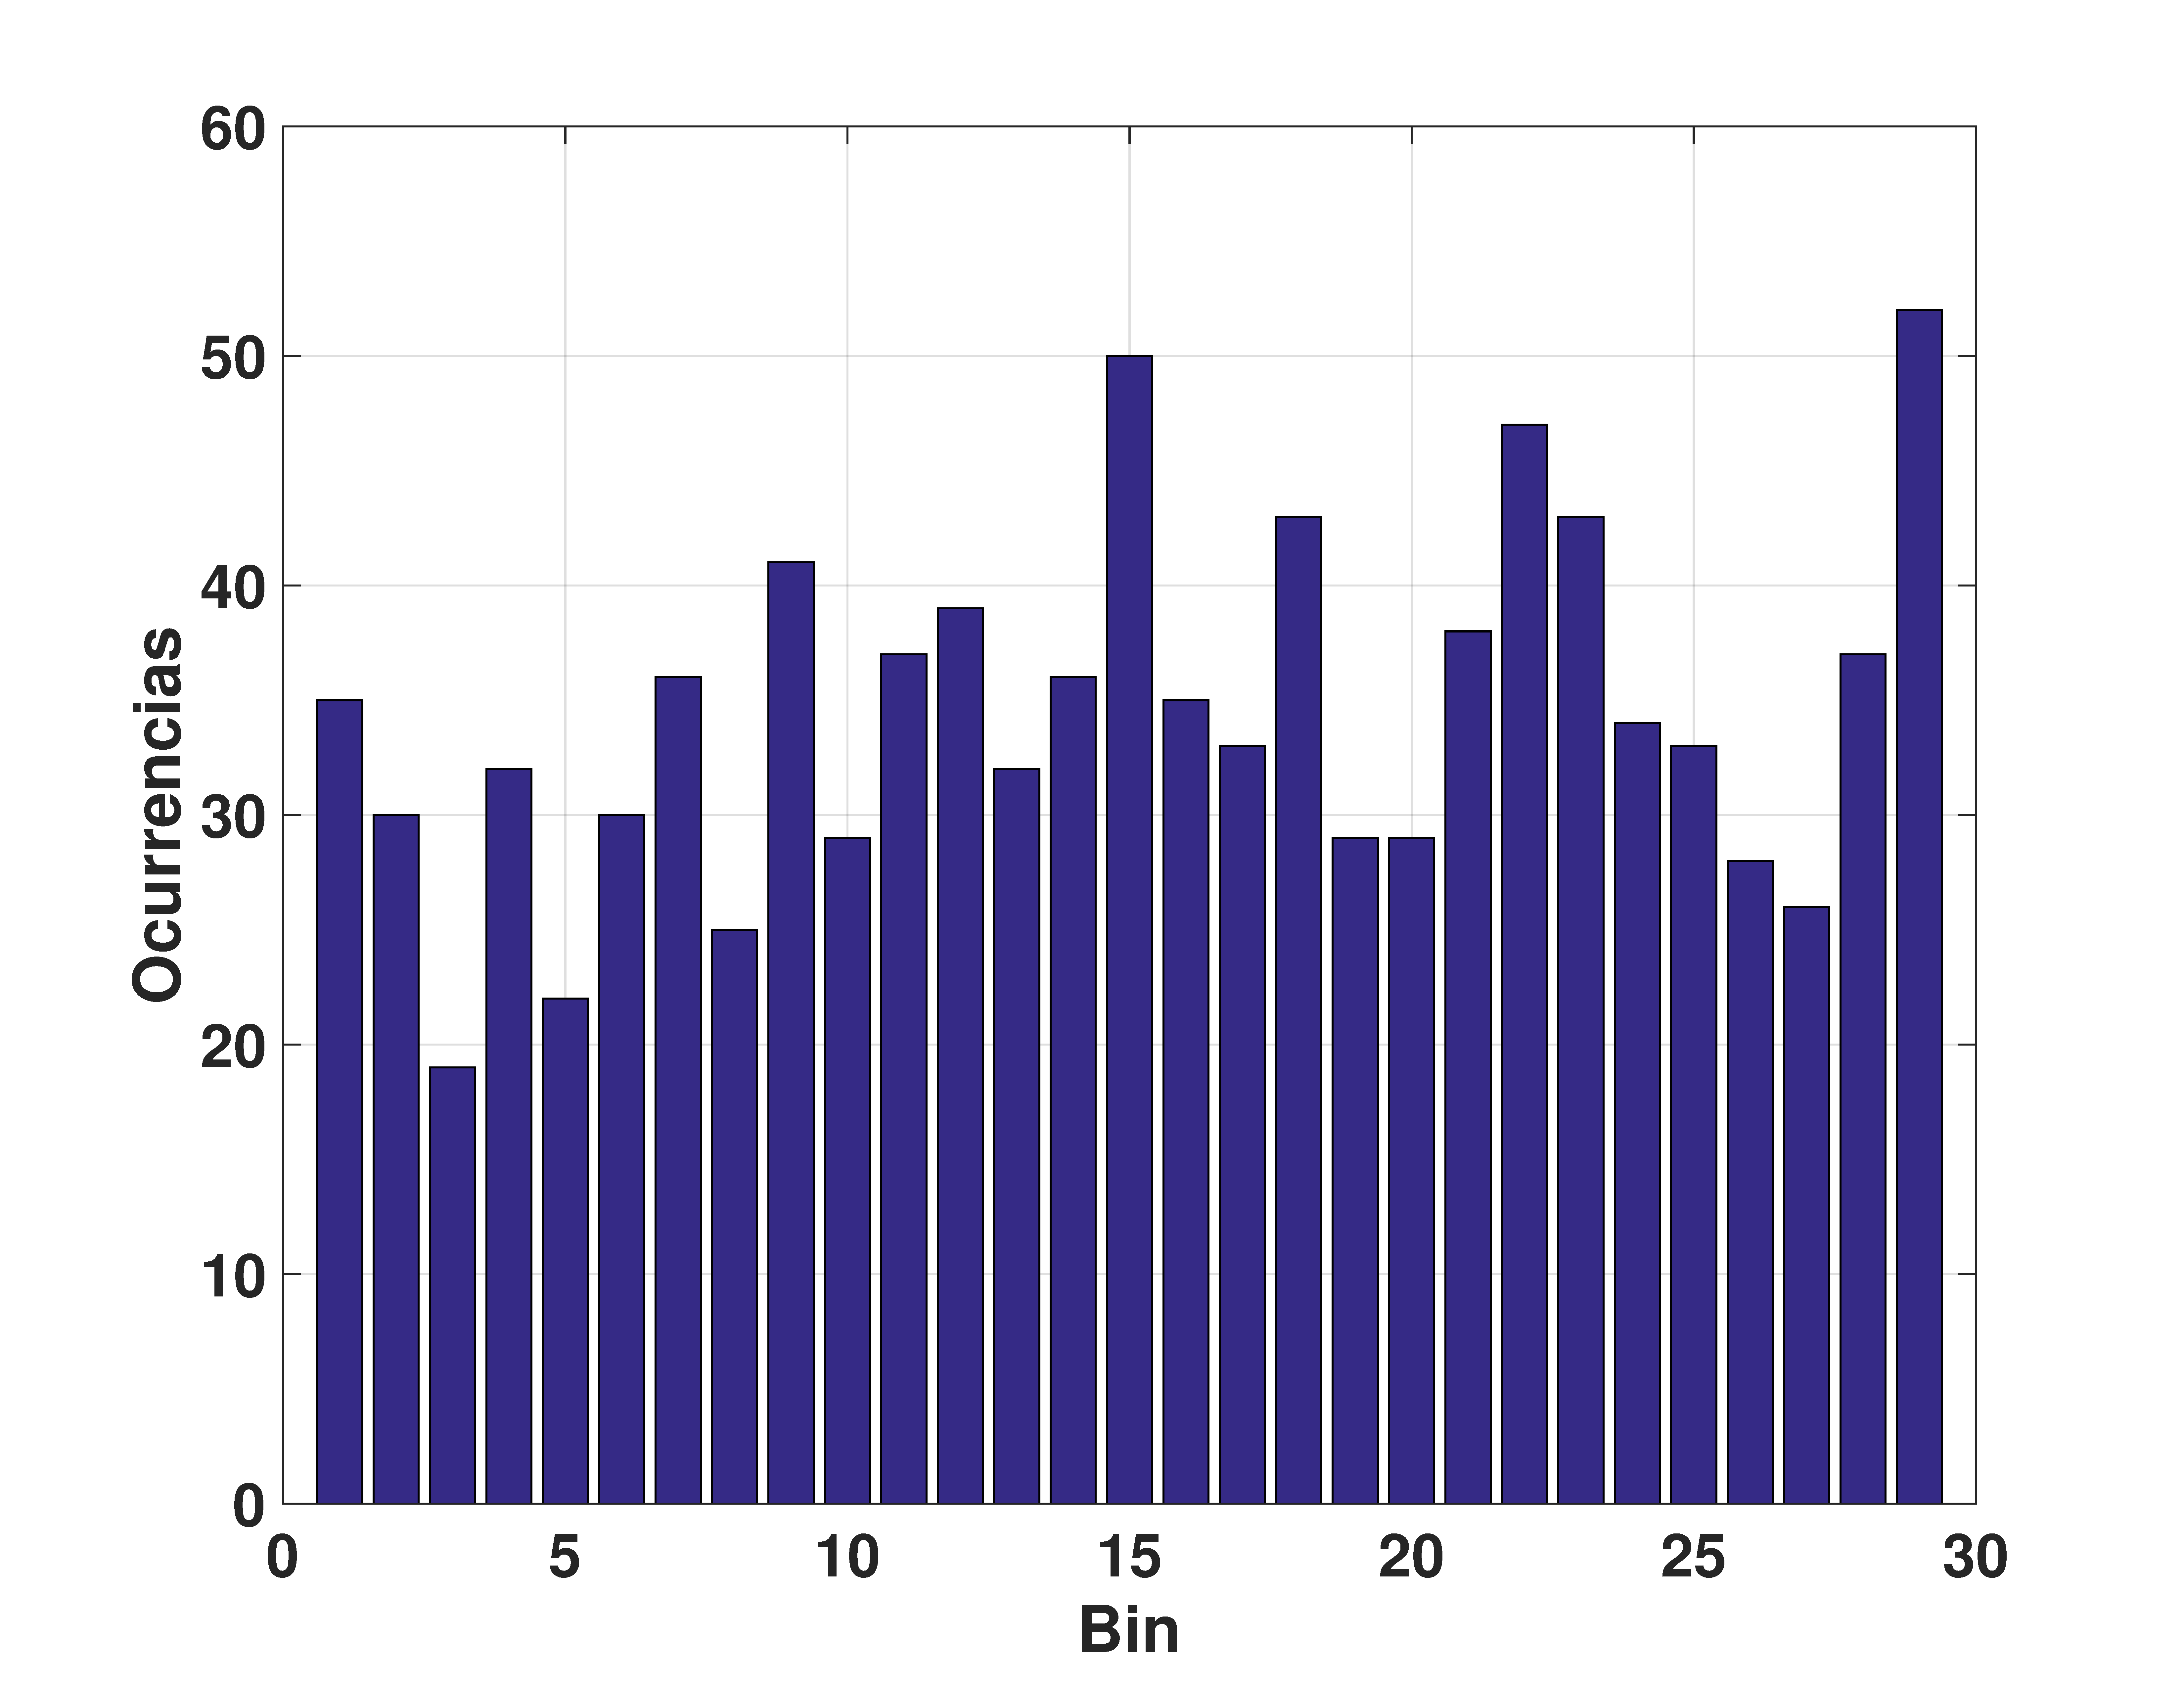
\includegraphics[width=\textwidth]{HistVal_x}
		\caption{Histograma de valores de los puntos sin ordenar}
		\label{subfig:causal_nocausal_HistValx}
	\end{subfigure}
	\begin{subfigure}[t]{0.49\textwidth}
		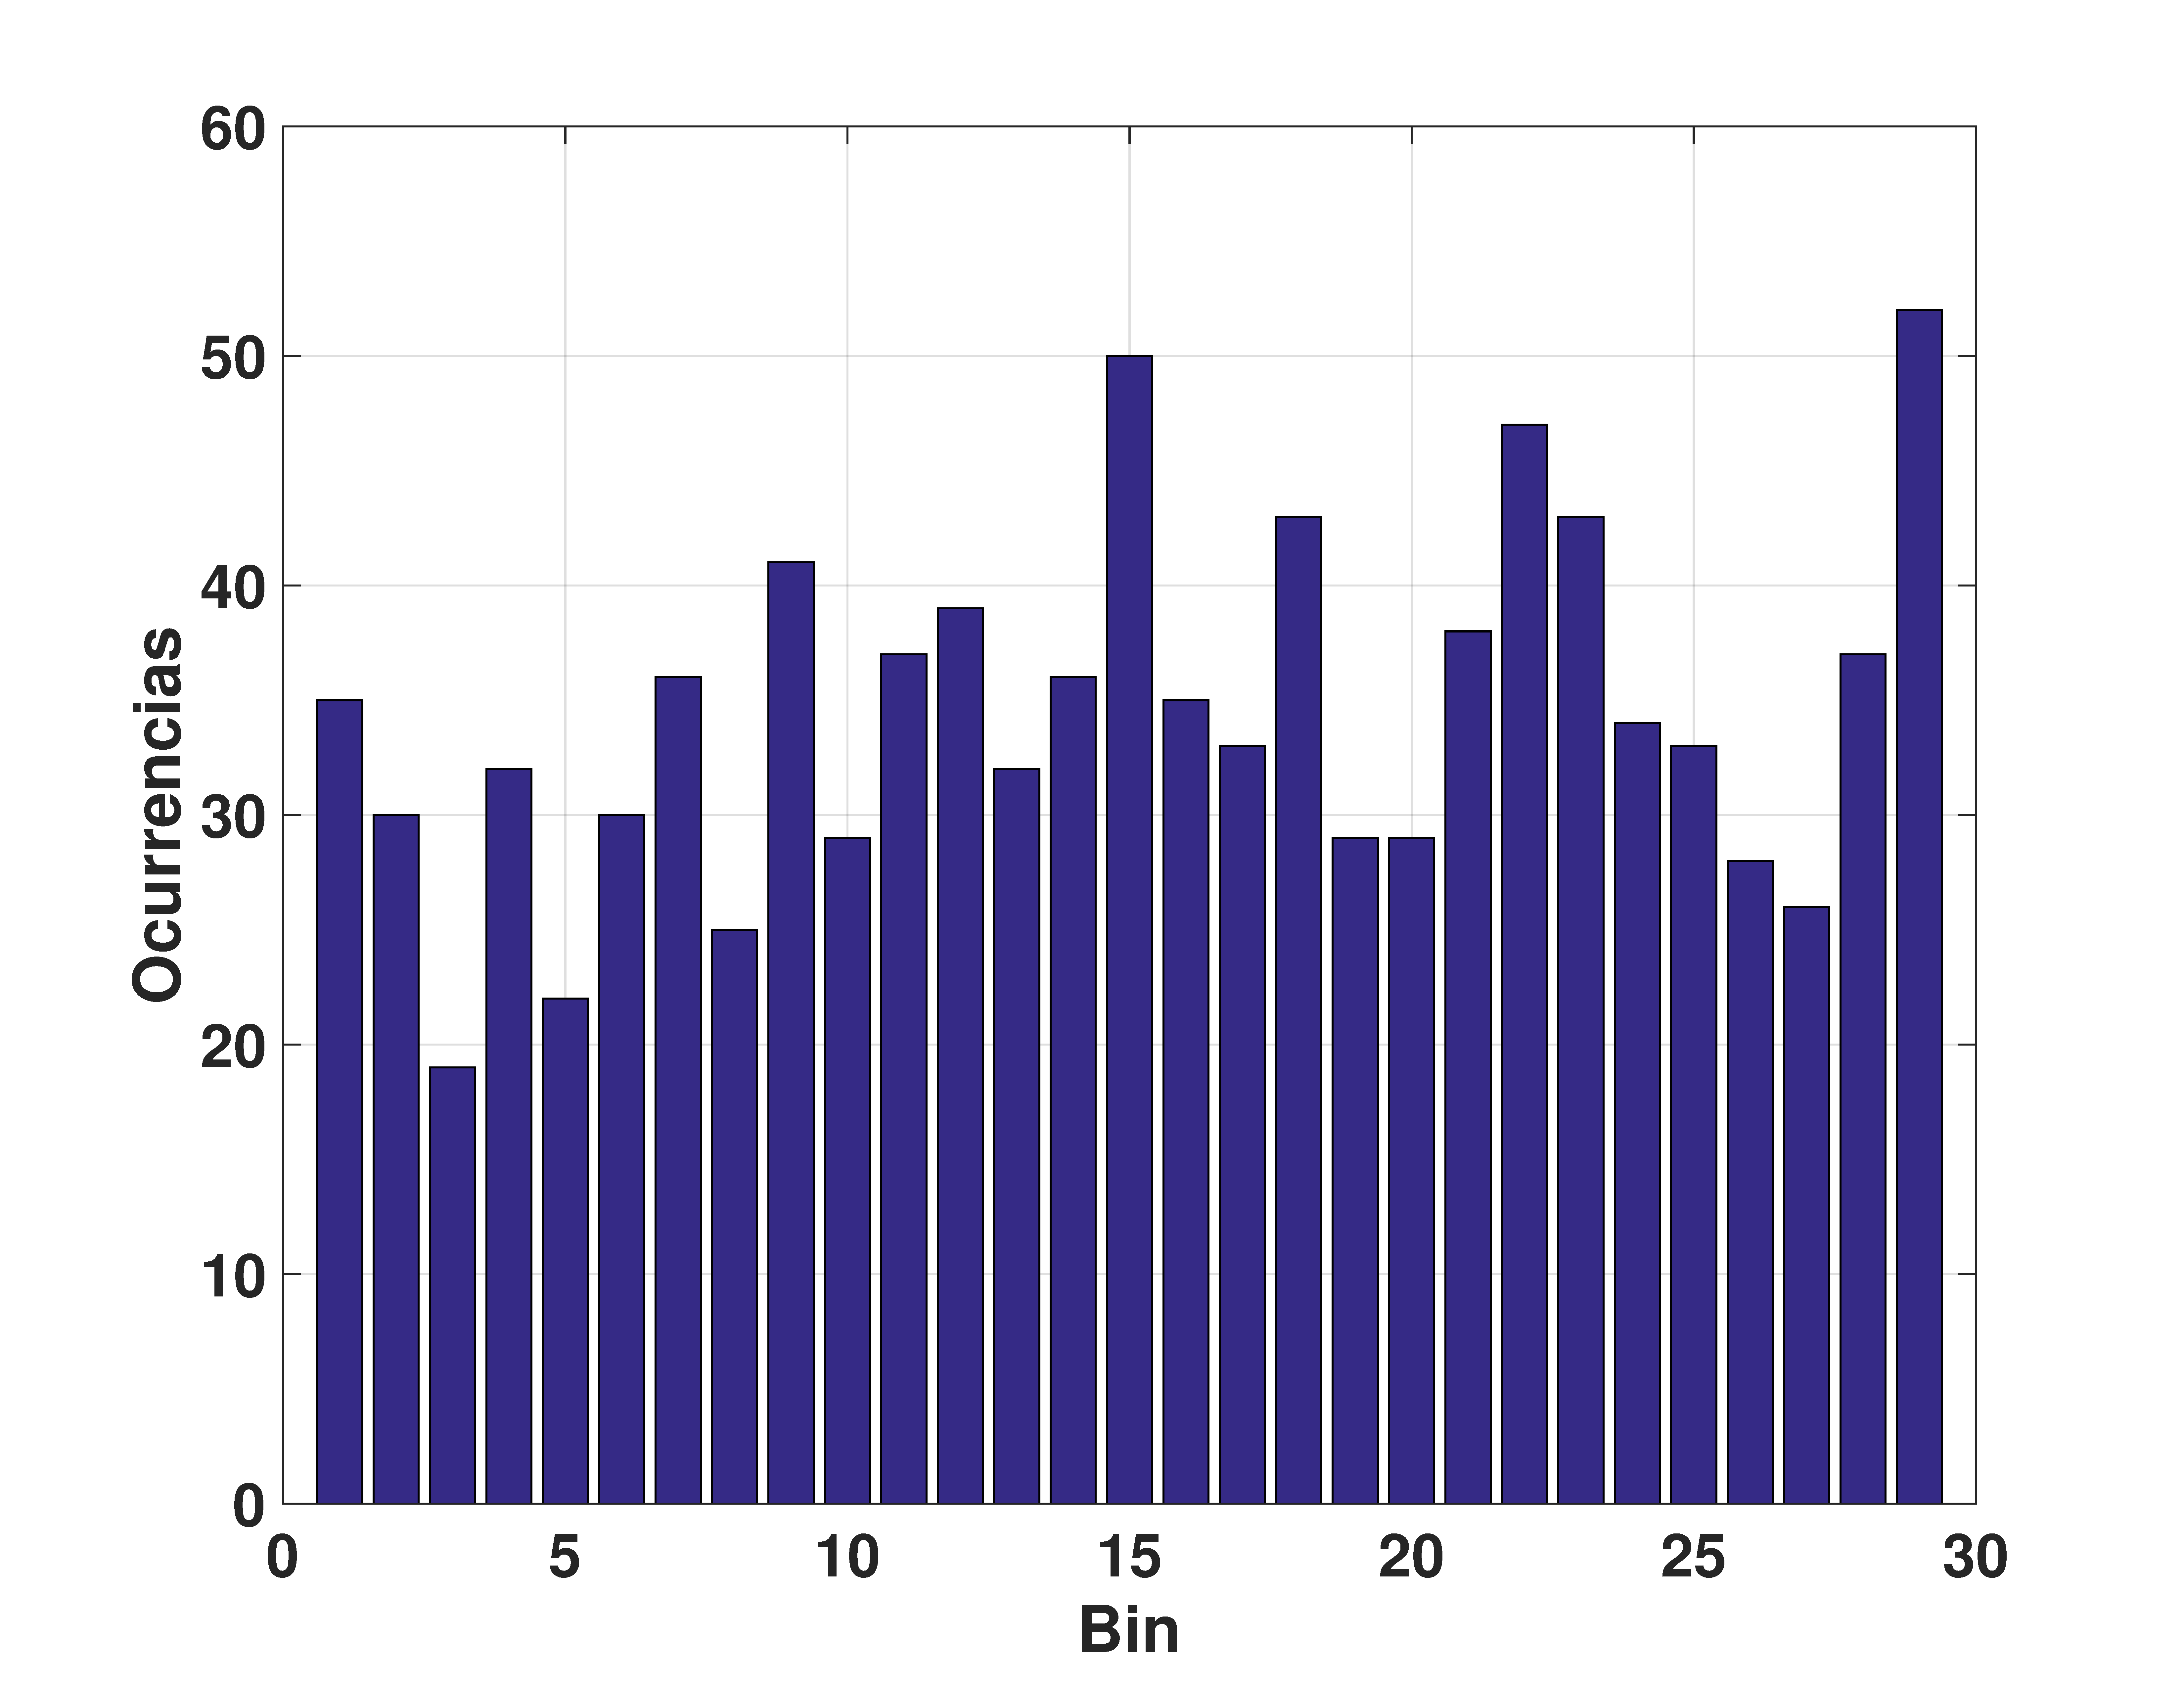
\includegraphics[width=\textwidth]{HistVal_y}
		\caption{Histograma de valores de los puntos ordenados}
		\label{subfig:causal_nocausal_HistValy}
	\end{subfigure}
	\begin{subfigure}[t]{0.49\textwidth}
		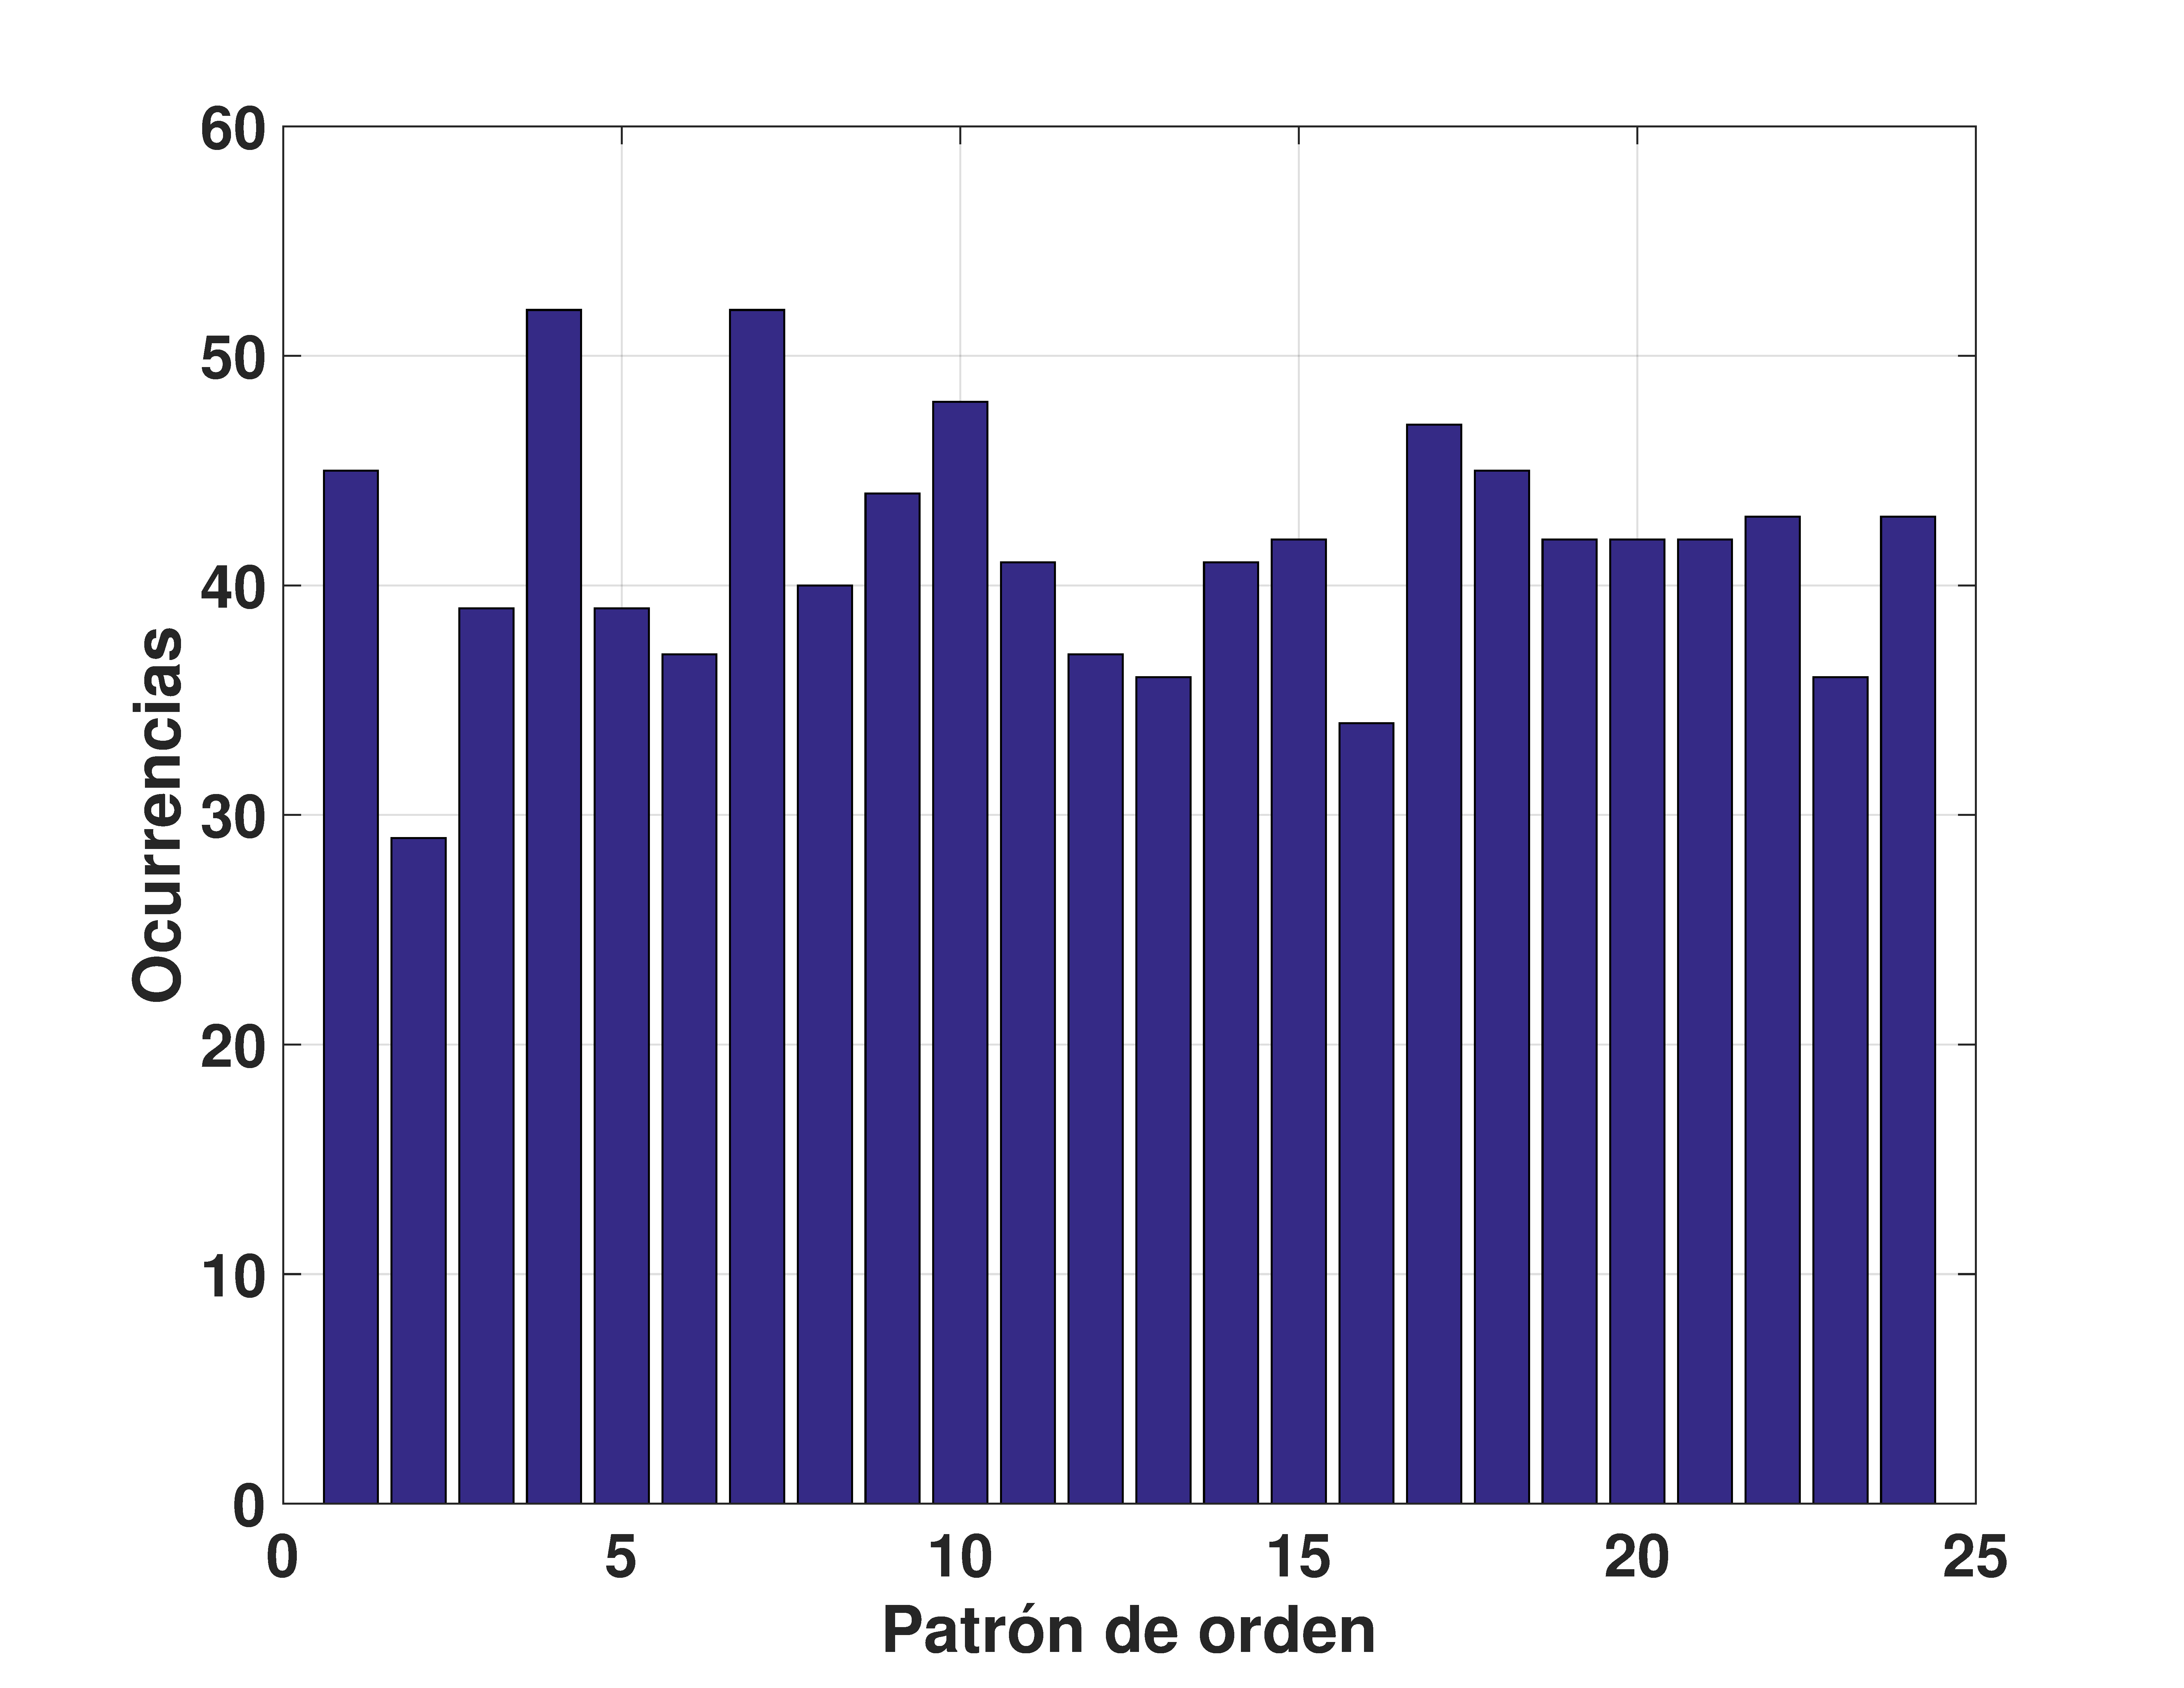
\includegraphics[width=\textwidth]{HistBP_x}
		\caption{Histograma de patrones de orden de los puntos sin ordenar}
		\label{subfig:causal_nocausal_HistBPx}
	\end{subfigure}
	\begin{subfigure}[t]{0.49\textwidth}
		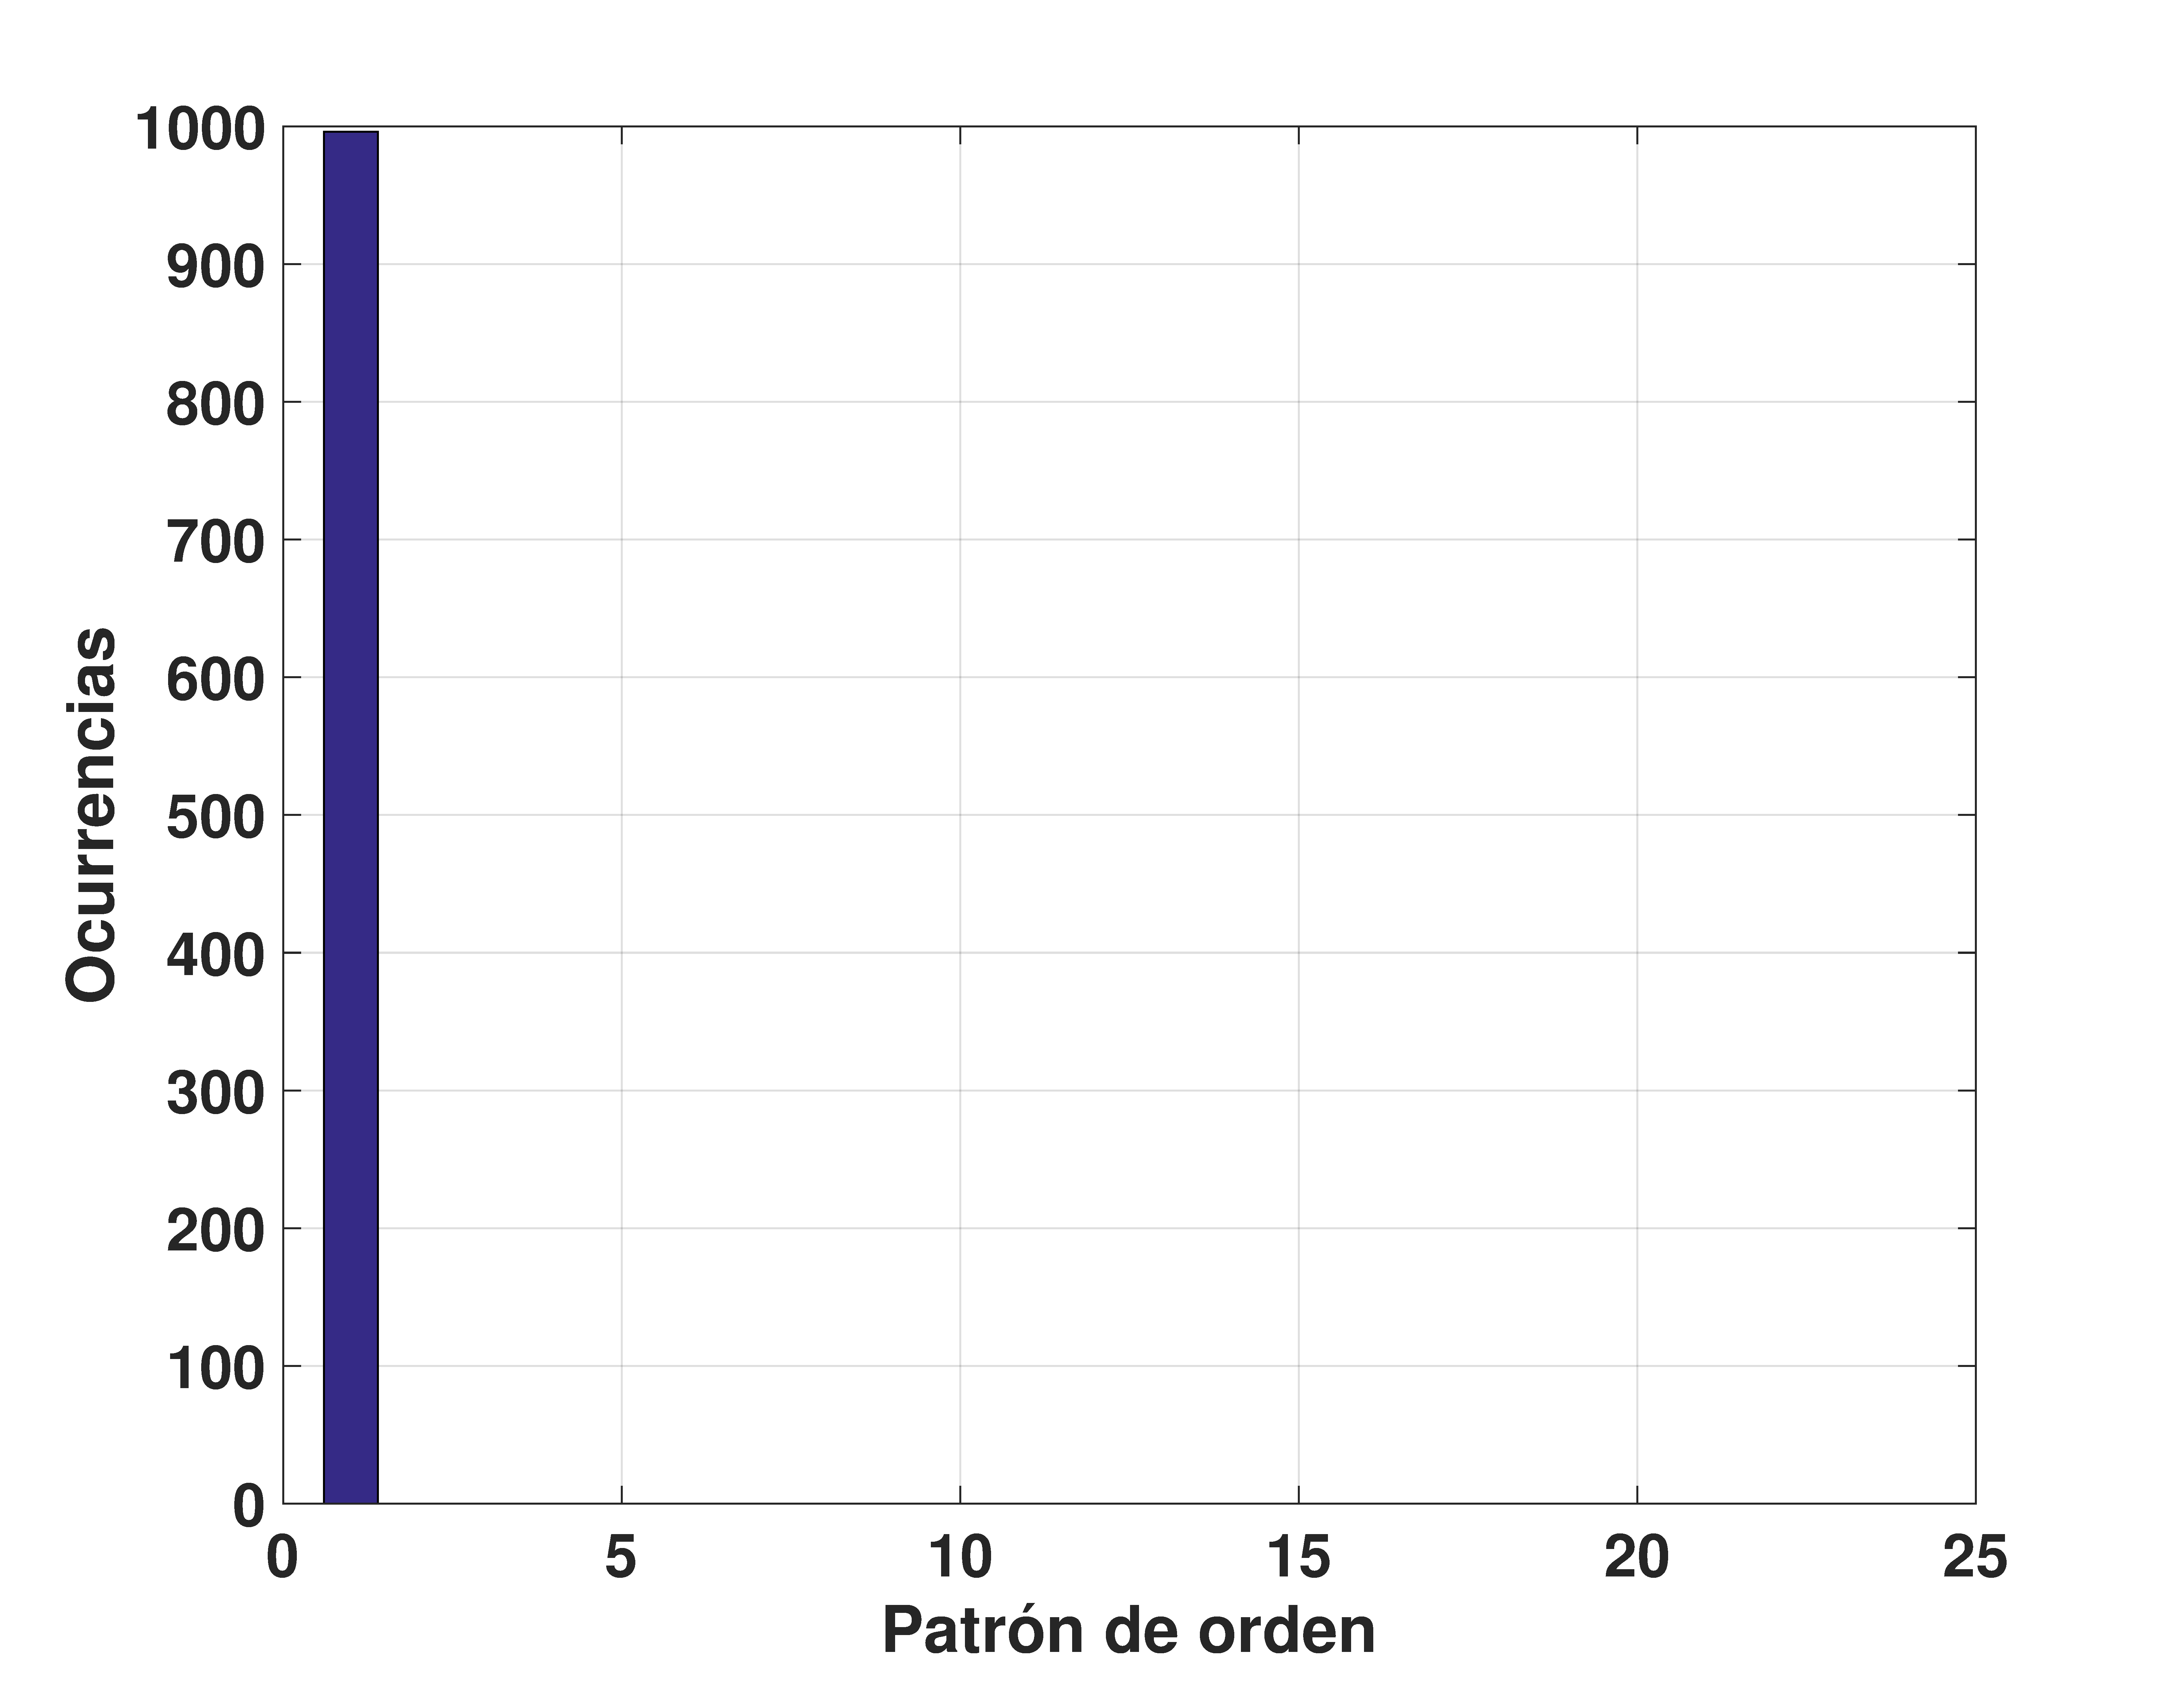
\includegraphics[width=\textwidth]{HistBP_y}
		\caption{Histograma de patrones de orden de los puntos ordenados}
		\label{subfig:causal_nocausal_HistBPy}
	\end{subfigure}
	\caption{Comparación entre histogramas causal y no causal}\label{fig:causal_nocausal}
\end{figure}

Recientemente, la entropía de permutación se amplió para incorporar también información de amplitud.
Ponderar las probabilidades de patrones individuales de acuerdo a su varianza mitiga los problemas potenciales con respecto a los patrones de "alto ruido, baja señal", porque los patrones de baja varianza que están fuertemente afectados por el ruido se ponderan en las distribuciones de patrones ordinales ponderados resultantes.
Por lo tanto, una posible desventaja de las estadísticas de los patrones ordinales, es decir, la pérdida de información de amplitud, se puede abordar mediante la introducción de pesos con el fin de obtener una "entropía de permutación ponderada (WPE)" \cite{Fadlallah2013}.
Los pesos no normalizados se calculan para cada ventana temporal para la serie de tiempo $X$, tal que
\begin{equation}
\label{WPE_weigth}
w_j~=~\frac{1}{D}\sum_{k=1}^{D} \left(x_{j+k-1}-\bar{X_j^D}\right)^2.
\end{equation}
En la ecuación anterior $x_{j+k-1}-\bar{X_j^D}$ denota la media aritmética del actual vector de embedding de longitud $D$ y su varianza $w_j$ se utiliza entonces para ponderar las frecuencias relativas de cada patrón ordinal $p_j$.
Originalmente, se propuso esta técnica para discriminar patrones sumergidos en un bajo nivel de ruido.
Nosotros también aprovechamos el hecho de que los puntos fijos no se computan en el WPE.

Al calcular la entropía de Shannon normalizada $H$ y la complejidad estadística $C$ de estas PDFs, y los valores obtenidos se denotan como:
\begin{itemize}
	\item $H_{hist}$, es la entropía de Shannon normalizada aplicada a una PDF no causal $P_{hist}$
	\item $H_{BP}$, es la entropía de Shannon normalizada aplicada a una PDF causal $P_{BP}$
	\item $H_{BPW}$,es la entropía de Shannon normalizada aplicada a una PDF causal con contribuciones de aplitud $P_{BPW}$
	\item $C_{BP}$, es la complejidad estadística normalizada aplicada a una PDF causal $P_{BP}$
	\item $C_{BPW}$, es la complejidad estadística normalizada aplicada a una PDF causal con contribuciones de amplitud $P_{BPW} $
\end{itemize}

\subsection{Planos doble entropía y entropía-complejidad}

Una visualización particularmente útil de los cuantificadores de la Teoría de la Información es su yuxtaposición en los gráficos bidimensionales.
Se definen cuatro planos de información:
\begin{enumerate}
	\item Entropía causal vs. entropía no-causal, $H_{BP} \times H_{hist}$
	\item Entropía causal con contribución de amplitudes vs. entropía no-causal, $H_{BPW} \times H_{hist}$
	\item Complejidad causal vs. entropía causal, $C_{BP} \times H_{BP}$
	\item Complejidad causal con contribución de amplitudes vs. entropía causal con contribución de amplitudes, $C_{BPW} \times H_{BPW}$
\end{enumerate}

Estas herramientas de diagnóstico demostraron ser particularmente eficientes para distinguir entre el caos determinista y la naturaleza estocástica de una serie de tiempo ya que los cuantificadores de permutación tienen comportamientos distintos para diferentes tipos de procesos.

En la Fig. \ref{fig: HH} se muestran los planos $H_ {BP} \times H_{hist}$ y $H_{BPW} \times H_{hist}$ colapsados en un mismo plano.
En este plano un valor más alto en cualquiera de las entropías, $H_{BP}$, $H_{BPW}$ o $H_{hist}$, implica una mayor uniformidad de la PDF implicada.
El punto $(1, 1)$ representa el caso ideal con histograma uniforme y distribución uniforme de los patrones de orden.
Mostramos algunos puntos relevantes como ejemplo.

El ruido aleatorio blanco ideal con distribución uniforme da un punto en $(H_{hist}, H_{BP}) = (1, 1)$ representado por un círculo azul, un círculo rojo en la misma posición muestra los resultados cuando se incluyen las contribuciones de amplitud $(H_{hist}, H_{BPW}) = (1, 1)$.
Si ordenamos el vector ideal con distribución uniforme de forma ascendente, los puntos resultantes se muestran con un cuadrado azul $(H_{hist}, H_{BP}) = (1, 0)$ y un cuadrado rojo $(H_{hist}, H_{BPW}) = (1, 0)$, este ejemplo ilustra la complementariedad de $H_{hist}$ y $H_{BP}$.

Las estrellas azules y rojas muestran $(H_{hist}, H_{BP})$ y $ (H_{hist}, H_{BPW})$ respectivamente aplicadas a una señal de diente de sierra.
Los valores están perfectamente distribuidos en todos los intervalos, pero sólo aparecen unos pocos patrones de orden, esto explica el alto $H_ {hist}$ y bajo $H_ {BP}$.
La frecuencia de aparición de patrones de baja amplitud es mayor que los patrones de alta amplitud, entonces la PDF con contribuciones de amplitud es más uniforme y $H_ {BPW}$ es un poco más alto que $H_ {BP}$.
Cuando la señal de diente de sierra está contaminada con ruido blanco, se incrementan $H_ {BP}$ y $H_ {BPW}$ como se muestra con triángulos azules y rojos.
Es evidente que aparecen nuevos patrones de orden y tanto $H_{BP}$ como $H_{BPW}$ muestran valores más altos que los casos no contaminados, sin embargo el incremento de $H_{BPW}$ es menor que $H_{BP}$ mostrando que la técnica de registrar contribuciones de amplitud añade alguna inmunidad al ruido.

Finalmente, se evaluaron los cuantificadores de una secuencia de un mapa logístico que converge a un punto fijo, en todos los casos la longitud del vector de datos permanece constante y la longitud de transitorio es variable.
Los resultados obtenidos sin las contribuciones de amplitud se representan en puntos azules, convergen a $(H_{hist}, H_{BP}) = (0, 0)$ a medida que la longitud de transitorio se hace más corta, sin embargo $H_{BPW}$ (puntos rojos) permanece constante para todos los casos.
El último punto en $(H_{hist}, H_{BP}) = (0, 0)$ corresponde a un vector de ceros, en este caso el histograma de patrones de orden con contribuciones de amplitud es también un vector nulo y $H_{BPW}$ no se puede calcular.
A través de este último ejemplo, mostramos que la convergencia a un punto fijo puede ser detectada por la información conjunta de $H_{BP}$ y $H_{BPW}$.

En la figura \ref{fig:HC} se muestra el plano causal $H_{BP} \times C_{BP}$.
Podemos ver que no toda la región $0 < H_{BP} < 1$, $0 < C_{BP} < 1$ es alcanzable, de hecho, para cualquier PDF los pares $(H, C)$ de valores posibles caen entre dos curvas extremas en el plano $H_{BP} \times C_{BP}$ \ cite {Anteneodo1996}.
Los mapas caóticos tienen entropía intermedia $H_{BP}$, mientras que su complejidad $C_{BP}$ alcanza valores mayores, muy cercanos a los del límite de complejidad superior \cite{Rosso2007, Olivares2012}.
Para procesos regulares, la entropía y la complejidad tienen valores pequeños, cercanos a cero.
Los procesos estocásticos no correlacionados se ubican en la localización planar asociada con $H_{BP}$ cerca de uno y $C_{BP}$ cerca de cero.
Los sistemas aleatorios ideales que tienen un Bandt \& Pompe PDF uniforme, están representados por el punto $(1,0)$ \ cite{Gonzalez2005} y una PDF tipo delta corresponde al punto $(0,0)$.

En la figura \ref{fig:HC} mostramos $H_{BP} \times C_{BP}$ con y sin contribuciones de amplitud.
Se muestran los mismos puntos de muestra para ilustrar las posiciones planas para diferentes vectores de datos.

En ambos planos de información $H_ {BP} \times H_ {hist}$ en la Fig. \ref{fig:HH} y $H_{BP} \times C_{BP}$ en Fig. \ref{fig:HC}, los datos estocásticos, caóticos y deterministas están claramente localizados en diferentes posiciones planares.

\begin{figure}[htpb]
	\centering	
	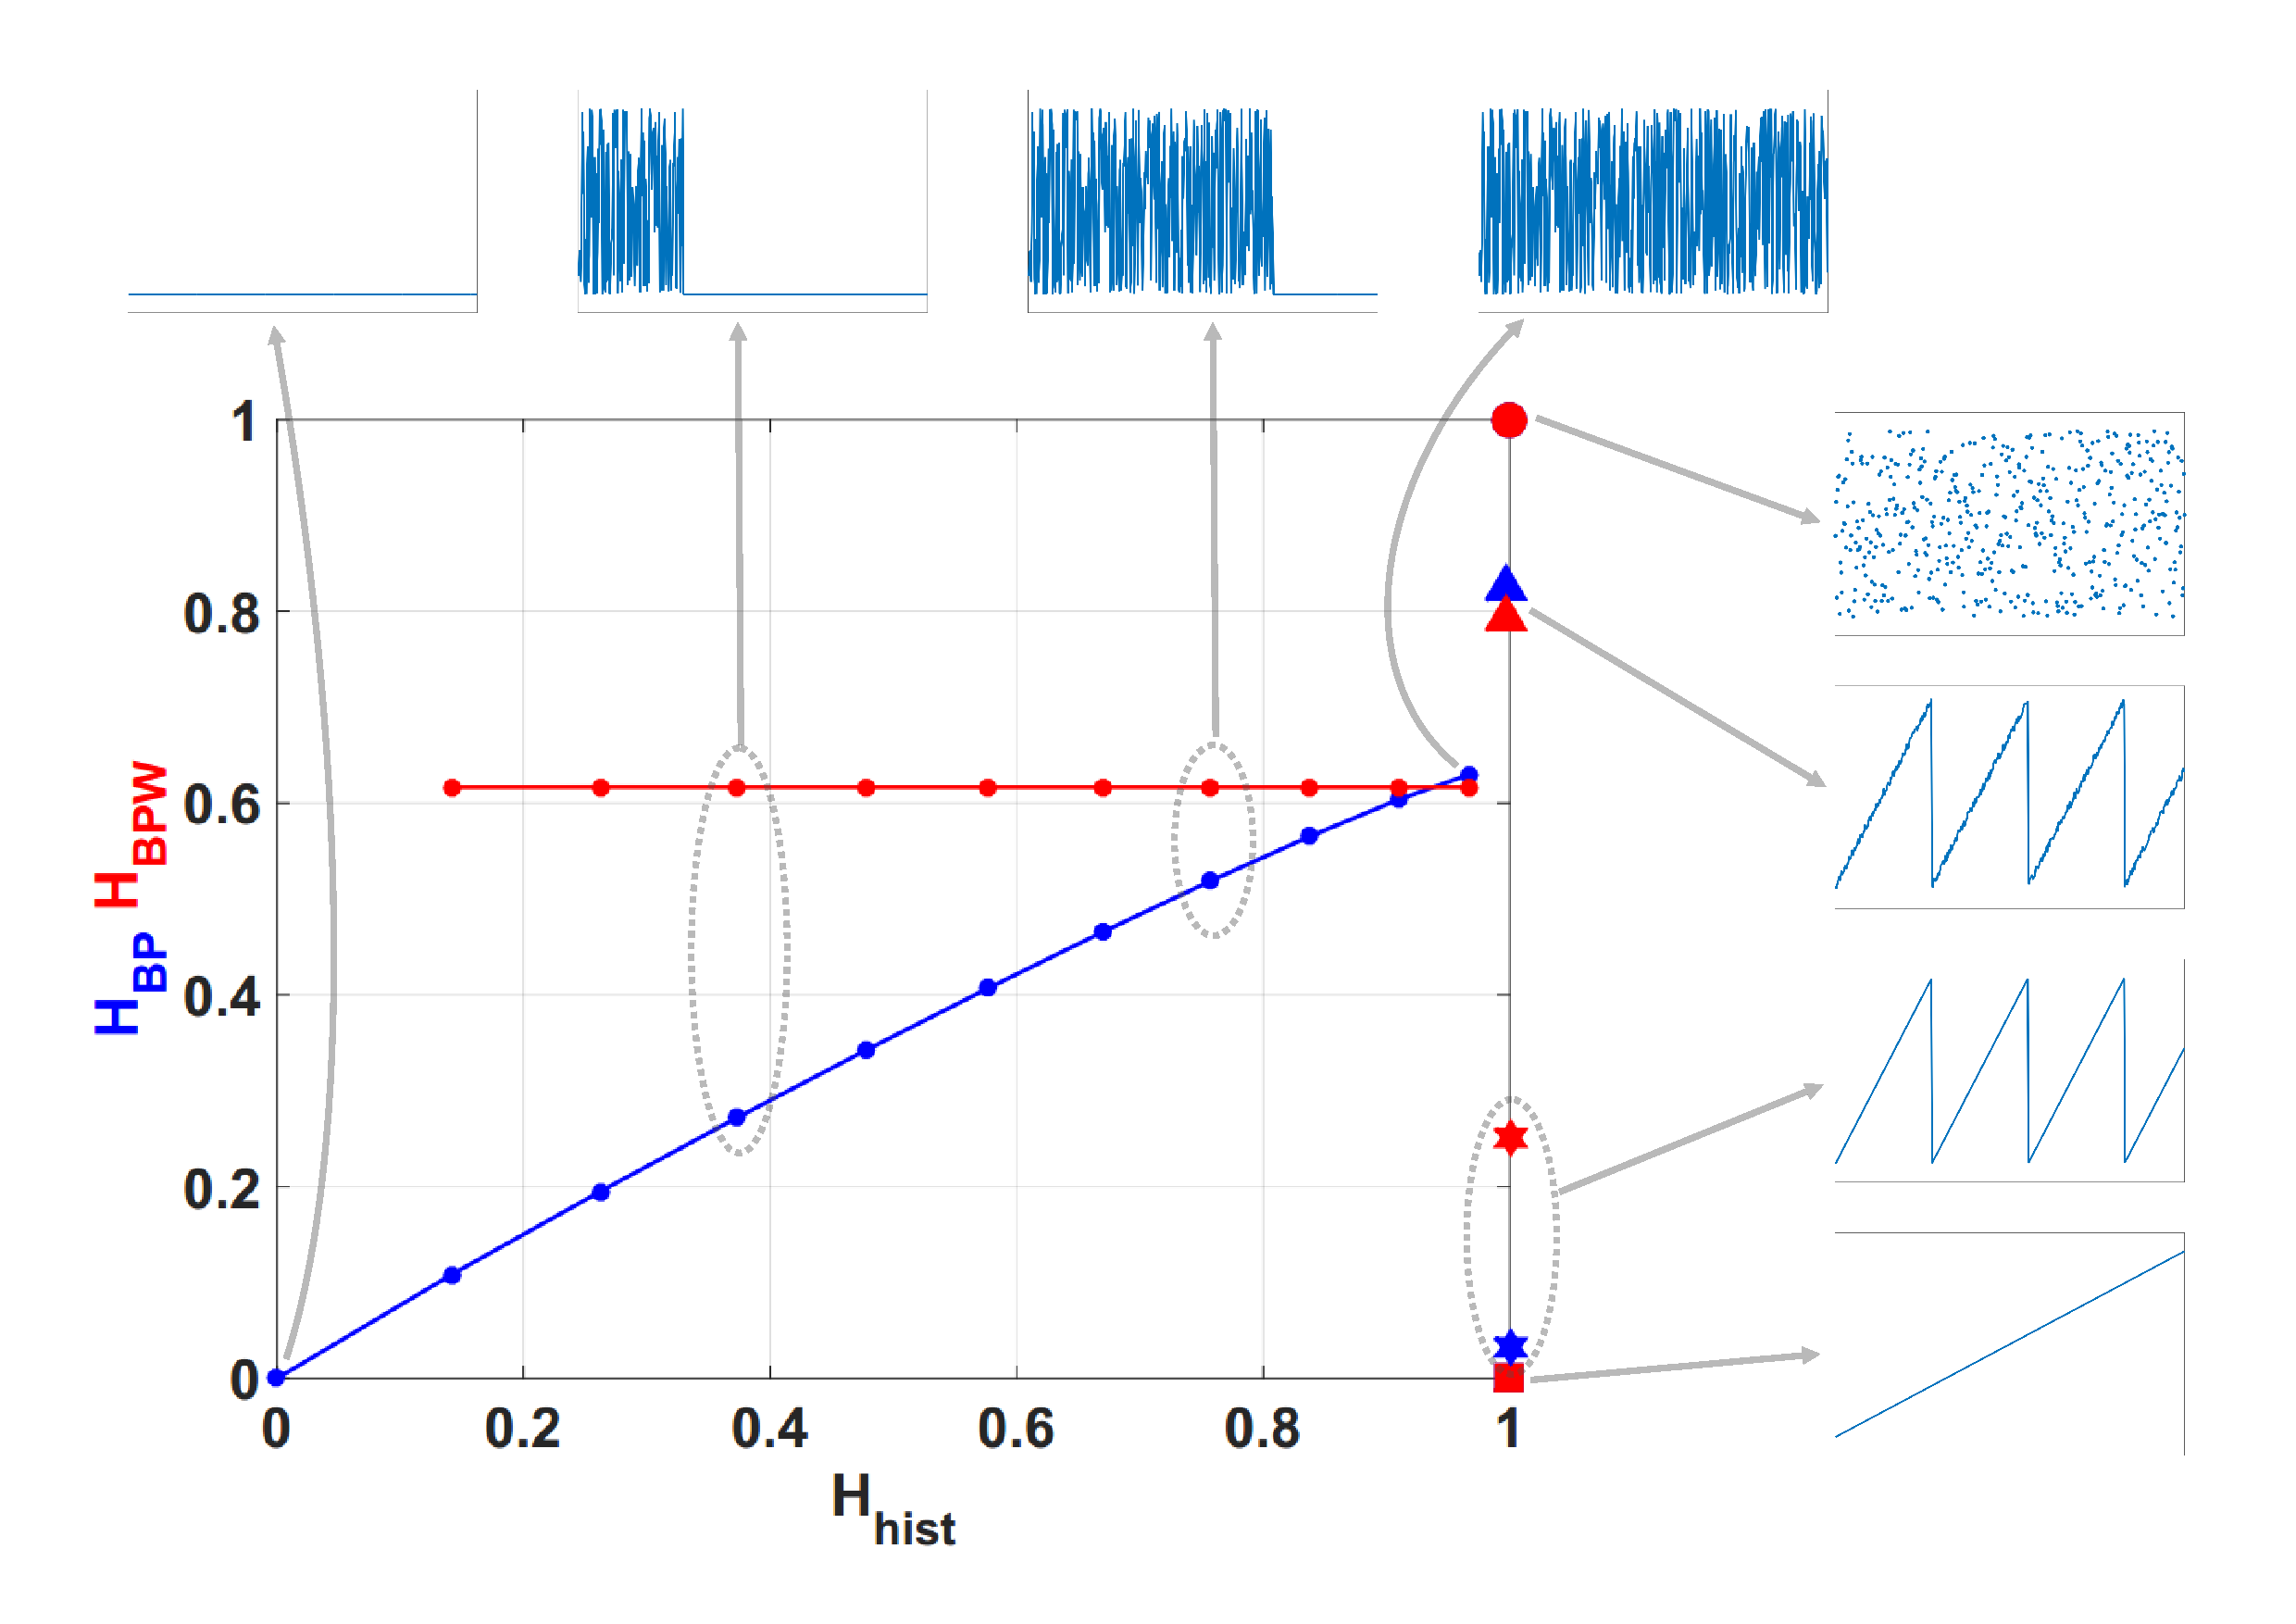
\includegraphics[width= .99\textwidth]{Fig1HHSignals}
	\caption{Causal-Non causal Entropy plane.}
	\label{fig:HH}
\end{figure}

\begin{figure}[htpb]
	\centering		
	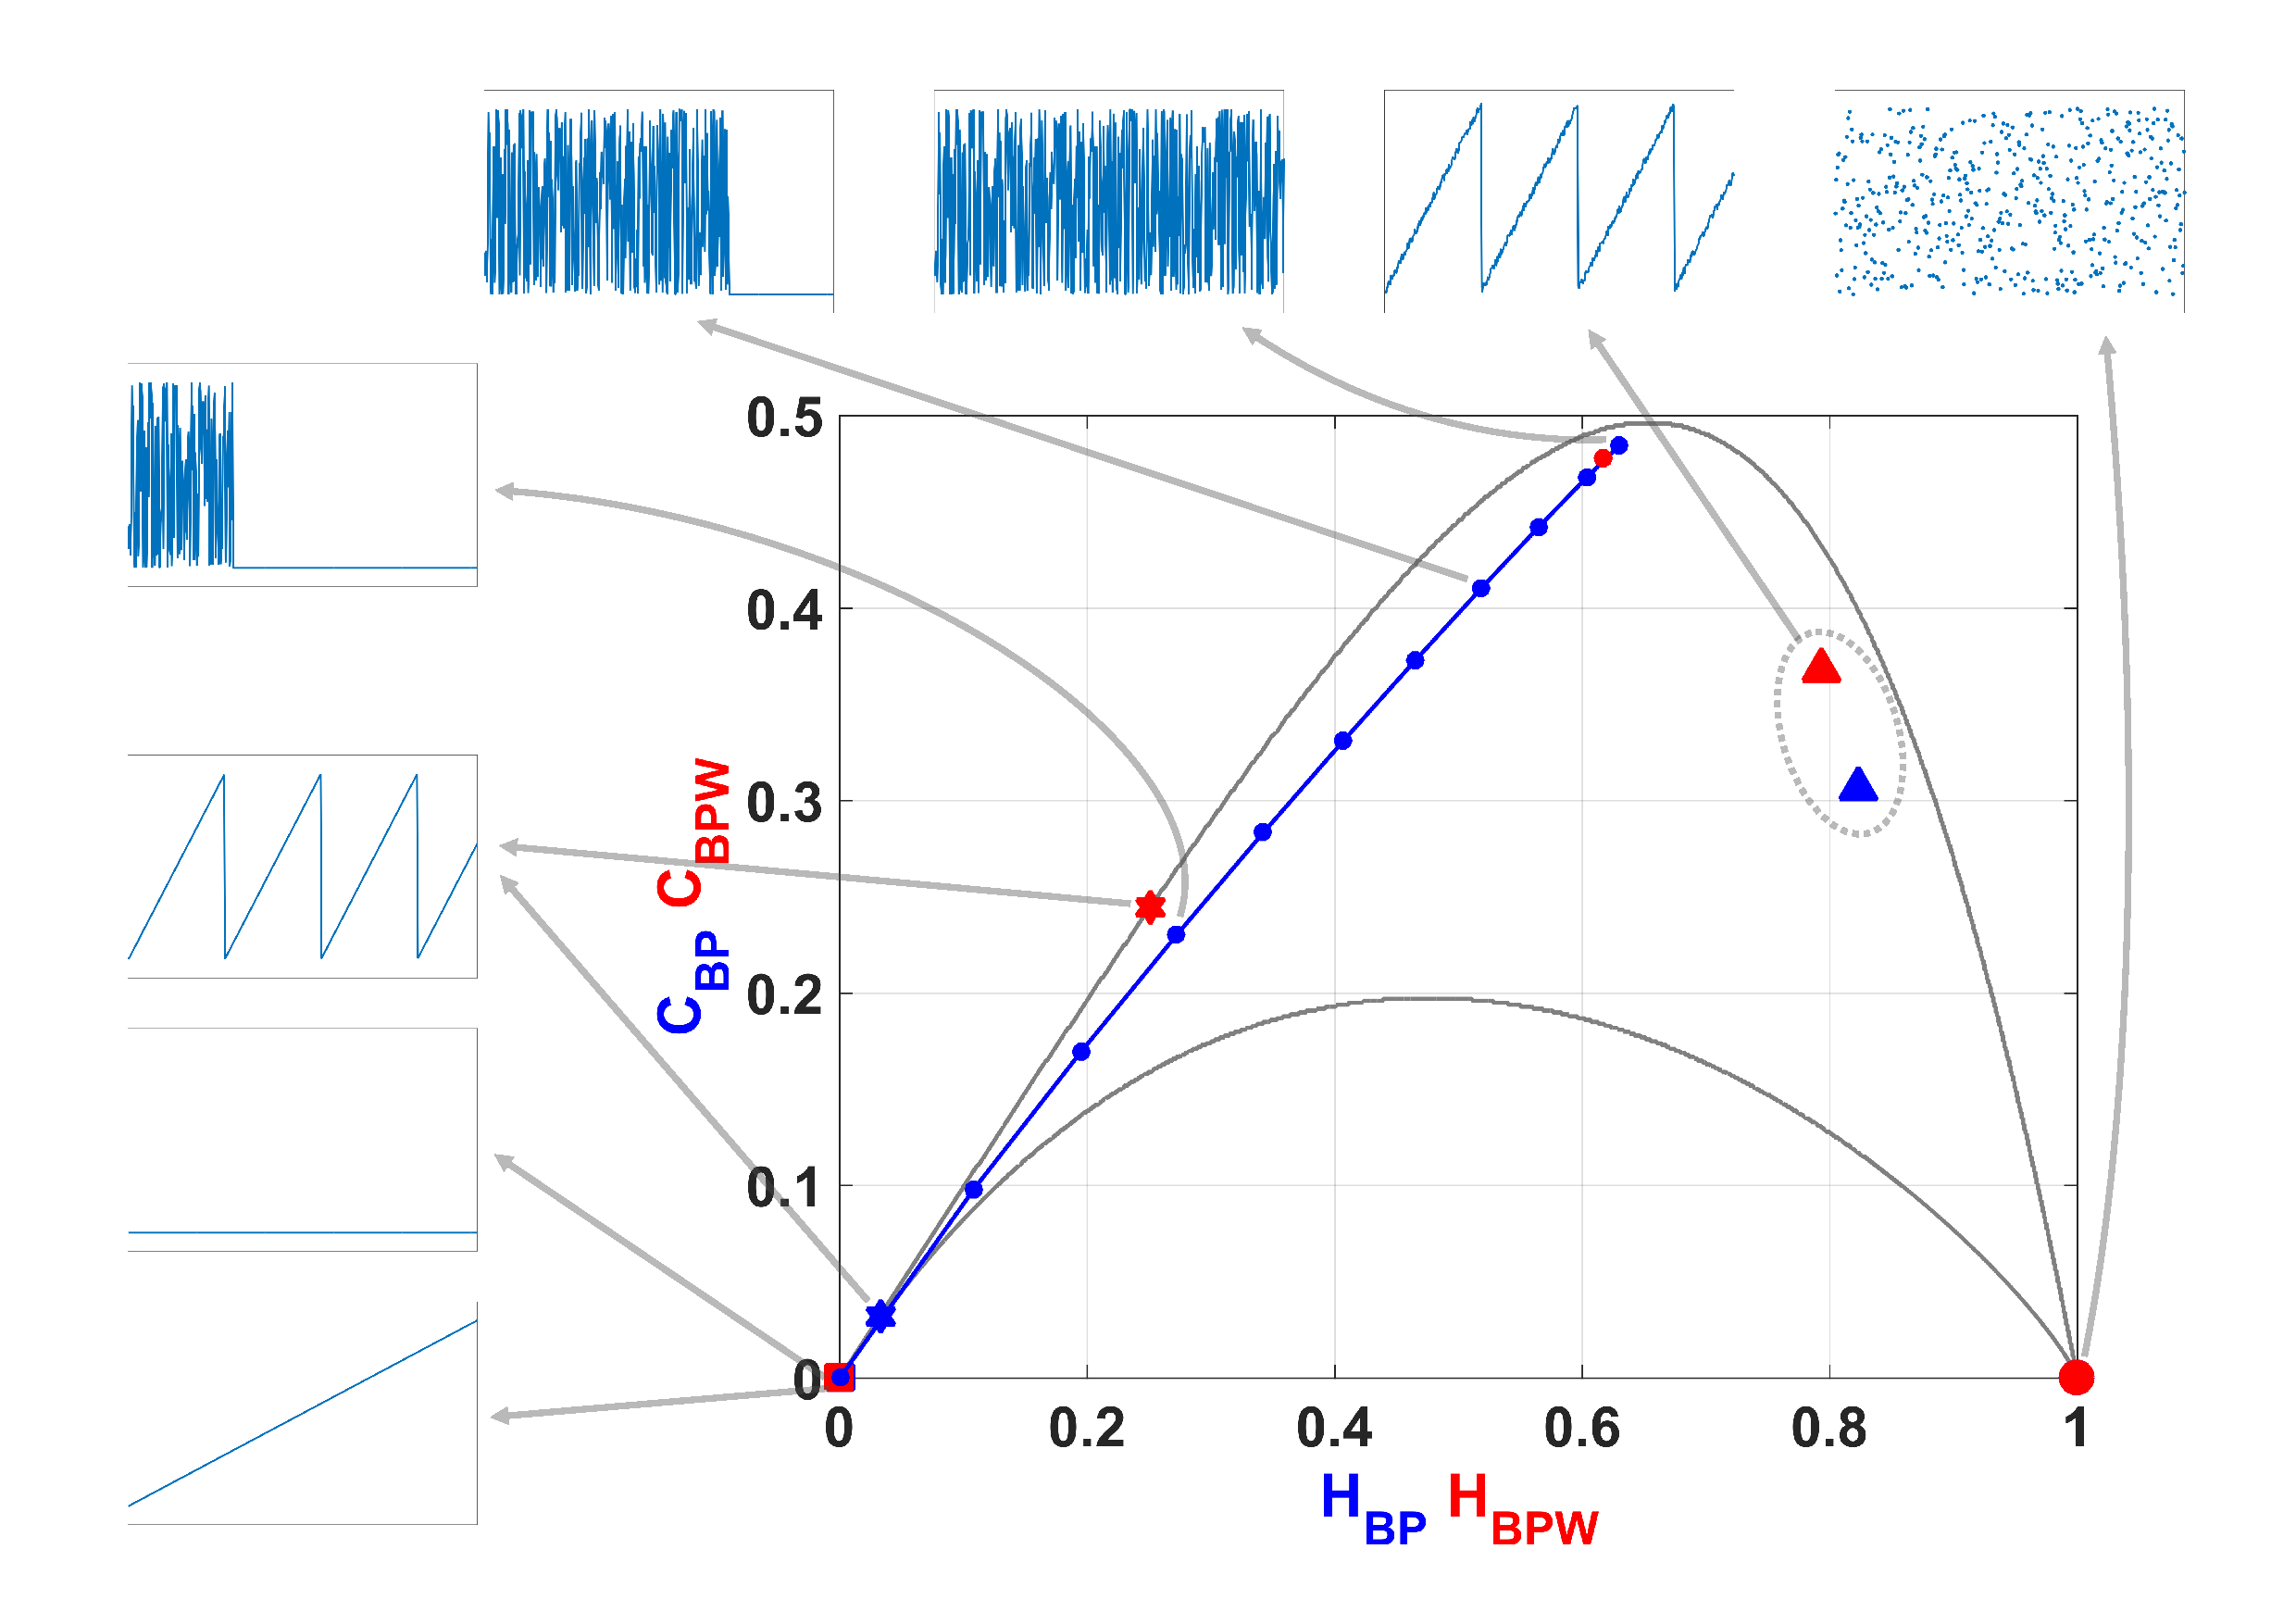
\includegraphics[width= .99\textwidth]{Fig1HCSignals}
	\caption{Causal Entropy-Complexity plane.}
	\label{fig:HC}
\end{figure}

También usamos el número de patrones perdidos MP como un cuantificador \cite {Rosso2012}.
Como mostraron recientemente Amigó y colaboradores \cite{Amigo2006,Amigo2007,Amigo2008,Amigo2010}, en el caso de mapas deterministas, no todos los patrones de orden posibles pueden materializarse efectivamente en órbitas.
De hecho, la existencia de estos patrones de orden faltantes se convierte en un hecho persistente que puede considerarse como una nueva propiedad dinámica.
Por lo tanto, para una longitud de patrón fija (dimensión de embedding $D$) el número de patrones perdidos de una serie temporal (patrones no observados) es independiente de la longitud de la serie $N$.
Obsérvese que esta independencia no caracteriza otras propiedades de la serie como la proximidad y la correlación \cite{Amigo2007,Amigo2010}.

\subsection{Entropías diferenciales}
\label{subsec:addquanti}

La entropía de Shannon $S(P)$ es el punto de partida para otros cuantificadores.

!!!!HABLAR DE LOS CONJUNTOS DE PARTICIONES Y NO SE QUE!!!

Para medir la entropía de una serie binaria es necesario 

!!!FIN DE HABLAR DE LOS CONJUNTOS DE PARTICIONES Y NO SE QUE!!!

\begin{enumerate}
	\item Entropía normalizada $H(P)$: es la entropía de Shannon dividida por su valor máximo. Por ejemplo, si usamos $S_2$ (ver arriba), se obtiene la entropía máxima para equiprobabilidad entre dos símbolos. Su valor es $S_{max}=-1/2 log(1/2)-1/2 log(1/2)=log(2)=1$; tentonces, la entropía normalizada es $H_2=S_2$. Si usamos $S_W$ la equiprobabilidad entre las $2^W$ posibles palabras (números decimales de $W$-bits) produce $S_{max}=W$ y $H_W=S_W/W$. Finalmente, para $S^{(D)}_{BP}$ la equiprobabilidad entre los $D!$ patrones de orden produce $S_{max}= log(D!)$ y $H^{(D)}_{BP}=S^D_{BP}/log(D!)$.
	\item Entropía diferencial o condicional $h$ y $h^*$ son:
	\begin{eqnarray}
	h~=~S_{W+1}-S_W\\
	h^*~=~S_{BP}^{(D+1)}-S_{BP}^{(D)}
	\end{eqnarray}
	En las expresiones de arriba $W=1,2,...$ y $D=2,3,...$, $S_0=0$ y $S_{BP}^{(1)}=0$. Esta entropía diferencial o condicional da la cantidad promedio de información requerida para predecir el símbolo $(W+1)$ (o $(D+1)$), dado los $W$ (o $D$) símbolos precedentes.
	\item Finalmente, las \emph{rate entropies} $h_0$ y $h_0^*$ \cite{Ebeling2001,Amigo2005} son dadas por:
	\begin{eqnarray}
	h_0=\lim\limits_{W\rightarrow \infty} h=\lim\limits_{W\rightarrow \infty}{S_{W}/W }\\
	h^*_0= \lim\limits_{D\rightarrow \infty} h^*=\lim\limits_{D\rightarrow \infty}{S^{(D)}_{BP}/(D-1)}
	\end{eqnarray}
\end{enumerate}

Enfatizemos algunas cuestiones importantes involucradas en los cálculos de las entropías binarias mencionadas anteriormente:
\begin{enumerate}
	\item La entropía binaria $S_2$ es no causal, mientras que ambas, la entropía de bloque $S_W$ y la entropía Bandt \& Pompe $S^{(D)}_{BP}$, son causales.
	\item La entropía de bloque $S_W$ tiene en cuenta las correlaciones entre $W$ bits consecutivos.
	La entropía Bandt \& Pompe $S^{(D)}_{BP}$ tiene en cuenta las correlaciones entre $D$ consecutivas palabras de longitud $W$.
	Ambos procedimientos de agrupación (números decimales de $W$ bits y patrones de permutación de $D$ números decimales) pueden realizarse con o sin superposición.
	La cantidad de datos requeridos para obtener buenas estadísticas es diferente dependiendo de que los procedimientos de agrupación se realicen.
	\item Para $ S_W $ solo hay un proceso de agrupación ($W$ bits agrupados para obtener una serie de números decimales $Y$).
	Definamos $\alpha$ como un parámetro de calidad estadística, dado por el cociente entre el número de elementos en la serie de tiempo simbólica $Y$ y la cantidad de símbolos en el alfabeto.
	En este documento, no aceptaremos $\alpha < 10$.
	
	Obviamente, el factor de calidad $\alpha$ aumenta con la longitud de la serie temporal:
	%
	\begin{enumerate}
		\item si el agrupamiento de $W$ bits está hecho con, dos palabras consecutivas de longitud $W$ comparten $W-2$ bits.
		En consecuencia, comenzando con un archivo con una longitud de $N$ bits obtenemos $N - W + 1$ palabras.
		Además, hay símbolos $2 ^ W$ en el alfabeto y $\alpha = (N - W + 1) / (2 ^ W)$.
		\item Si $S_W$ se evalúa sin superposición la cantidad de palabras de longitud $W$ es $floor\{N/W\}$ y el parámetro de calidad se calcula como $\alpha=floor~\{N/W\}/(2^W)$.
		Si $N \gg W$ el factor de calidad estadística es $W$ veces más bajo que el usado con superposición.
	\end{enumerate}
	
	\item En el caso de $S^{(D)}_{BP} $, hay dos procesos de agrupación involucrados.
	\begin{enumerate}
		\item Si ambos procesos de agrupamiento se realizan con superposición obtenemos $NW-D + 2$ elementos comenzando con un archivo $ N $ bits de longitud, y el factor de calidad es $\alpha = (NW-D + 2) / D!$.
		En este caso $S ^ {(D)}_{BP}$ tiene en cuenta las correlaciones entre $W + D$ bits consecutivos.
		\item Si el proceso de agrupación de $W$ bits se realiza sin superposición pero la agrupación de números decimales $D$ se realiza con superposición obtenemos $floor\{N/W\}-D+1$ elementos y el parámetro de calidad estadística es $\alpha=(floor\{N/W\}-D+1)/D!$.
		En este caso $S^{(D)}_{BP}$ incluirá correlaciones entre $WD$ bits consecutivos.
		\item Si el proceso de agrupación de $W$ bits se realiza con superposición y la agrupación de números decimales $D$ se realiza sin superposición, obtenemos $floor\{(N-W+1)/D\}$ elementos a partir de un archivo de $N$ bits.
		El factor de calidad estadística es $\alpha=floor\{(N-W+1)/D\}/D!$ y $S^{(D)}_{BP}$ tiene en cuenta correlaciones de $W+D-1$ bits.
		\item Si ambos procesos de agrupación se realizan sin superposición, obtenemos $floor\{floor\{N/W\}/D\}$ elementos a partir de un archivo de longitud de  $N$ bits.
		El factor de calidad estadística es $\alpha=floor\{floor\{N/W\}/D\}/D!$ y $S^{(D)}_{BP}$ tiene en cuenta las correlaciones entre $WD$ bits consecutivos.
	\end{enumerate}
\end{enumerate} 